
%\documentclass[manuscript,endfloat]{geophysics}
\documentclass[revised,endfloat]{geophysics}
%\documentclass[twocolumn,endfloat]{geophysics}

\usepackage{xy}
\usepackage{natbib}
\usepackage{graphicx}
\usepackage{url}
\usepackage{rotating}
\usepackage{lscape}
\usepackage{color}
\usepackage{rotating}
\usepackage{amsmath}
\usepackage{mathrsfs}
\usepackage{amssymb}      
\usepackage{algorithm}
\usepackage{algpseudocode}
\usepackage{booktabs}
\setcounter{MaxMatrixCols}{20}

\setlength\parindent{0pt}

\setlength\heavyrulewidth{0.25ex}

\DeclareGraphicsExtensions{.pdf}
\DeclareMathAlphabet\mathbfcal{OMS}{cmsy}{b}{n}
\DeclareMathOperator*{\argmin}{arg\,min}

\begin{document}

\title{SeisAcoustic}
\renewcommand{\thefootnote}{\fnsymbol{footnote}}

\address{
\footnotemark[1]Department of Physics,\\
University of Alberta, \\
Edmonton, Alberta, Canada. \\}

\author{Wenlei Gao\footnotemark[1]} 

\maketitle

%%%%%%%%%%%%%%%%%%%%%%%%%%%%%%%%%%%%%%%%%%%%%%%%%%%%%%%%%%%%%%%%%%%%%%%%%%%%%%
% ABSTRACT                                                                   %
%%%%%%%%%%%%%%%%%%%%%%%%%%%%%%%%%%%%%%%%%%%%%%%%%%%%%%%%%%%%%%%%%%%%%%%%%%%%%%


\begin{abstract}
Acoustic wave field modelling and inversion
\end{abstract}


%%%%%%%%%%%%%%%%%%%%%%%%%%%%%%%%%%%%%%%%%%%%%%%%%%%%%%%%%%%%%%%%%%%%%%%%%%%%%%
% INTRODUCTION                                                                   %
%%%%%%%%%%%%%%%%%%%%%%%%%%%%%%%%%%%%%%%%%%%%%%%%%%%%%%%%%%%%%%%%%%%%%%%%%%%%%%
\section{Method}
Our derivation start from the first-order acoustic wave equation which support variable density
\begin{equation}
\begin{split}
\frac{\partial v_z}{\partial t} &= b \frac{\partial p}{\partial z}   \\
\frac{\partial v_x}{\partial t} &= b \frac{\partial p}{\partial x} \\
\frac{\partial p}{\partial t} &= k(\frac{\partial v_z}{\partial z} + \frac{\partial v_x}{\partial x}) + f(t)\\
 \\
\end{split}, 
\label{eq1}
\end{equation}
where $b$ is buoyancy, the reciprocal of density $\rho$, $k$ is bulk modulus ($k = \rho v^2$), $v_z$ and $v_x$ are vertical and horizontal particle velocities and $p$ is pressure. $f(t)$ is additive source term. To eliminate undesirable boundary reflections, we implement PML absorbing boundary conditions. The pressure component $p$ is split into two unphysical components $p_z$ and $p_x$, where $p = p_z + p_x$. Equation \ref{eq1} can be reformulated as
\begin{equation}
\begin{split}
\frac{\partial v_z}{\partial t} + r_z\, v_z &= b \frac{\partial \left( p_z + p_x \right) }{\partial z}   \\
\frac{\partial v_x}{\partial t} + r_x\, v_x &= b \frac{\partial \left( p_z + p_x \right) }{\partial x}   \\
\frac{\partial p_z}{\partial t} + r_z\, p_z &= k \frac{\partial v_z}{\partial z} \\
\frac{\partial p_x}{\partial t} + r_x\, p_x &= k \frac{\partial v_x}{\partial x} + f(t)
\end{split}.  
\label{eq2}
\end{equation}
As the source term is additive, it can be added to either one of the last two equations. $\gamma_z$ and $\gamma_x$ are the PML damping coefficients in vertical and horizontal directions, respectively. The bulk modulus is set to $0$ when free surface boundary condition is implemented for the top boundary.

\subsection{Discretization of Acoustic wave equation}

We use stagger grid finite difference method to discretize equation \ref{eq2}, the particle $v_z$ is put on the stagger grid $[i+\frac{1}{2},j,it]$, horizontal particle velocity $v_x$ is put on the stagger grid $[i, j+\frac{1}{2}, it]$, and the pressure component is put on the grid $[i,j,it+\frac{1}{2}]$. Where $i,j,it$ are the grid index in vertical, horizontal, time directions, respectively. Figure \ref{f1} shows the locations of wave field components and model parameters, respectively.
\begin{figure}[htb] 
   \centering
   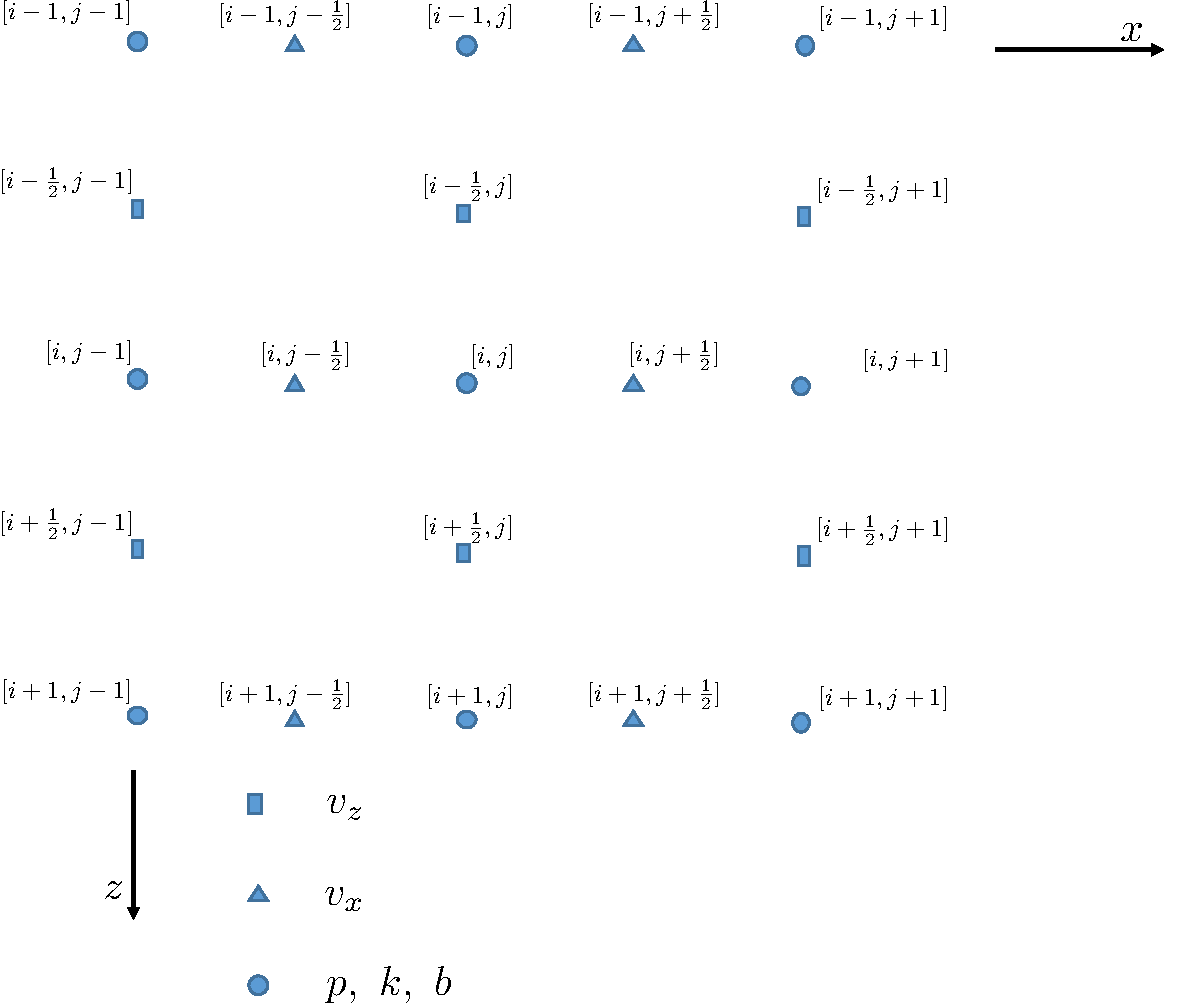
\includegraphics[width=0.6\columnwidth]{Fig/f1.pdf} 
   \caption{Stagger grid}
   \label{f1}
\end{figure}

\subsection{${\bf v}_z$ time stepping}
\begin{equation}
\frac{\partial v_z}{\partial t} + \gamma_z \, v_z = b \frac{\partial p}{\partial z}
\label{eq3}.
\end{equation}
The time partial derivative operator $\frac{\partial }{\partial t}$ is approximated by second-order central finite difference and spatial partial derivative operator is approximated by $2N^{th}$-order central finite difference. The center of both side of the equation is on $[i+\frac{1}{2},j,it+\frac{1}{2}]$. 
\begin{equation}
\begin{split}
&\frac{v_z[i+\frac{1}{2},j,it+1] - v_z[i+\frac{1}{2},j,it]}{dt} + \gamma_z[i+\frac{1}{2}]
\frac{v_z[i+\frac{1}{2},j,it+1] + v_z[i+\frac{1}{2},j,it]}{2}  \\
&= b[i+\frac{1}{2},j] \left( \frac{1}{dz} \sum_{n=1}^N  a_n \left( p[i+n,j,it+\frac{1}{2}] - p[i-n+1,j,it+\frac{1}{2}] \right) \right)
\end{split},
\label{eq4}
\end{equation}
where $dt$ is the time step size and $dz$ is the grid size in vertical direction. $b[i+\frac{1}{2},j]$ is approximated by averaging the buoyancy on neighbouring two grid points, so $b[i+\frac{1}{2},j] = (b[i,j] + b[i+1,j]) / 2 $. $a_n$ is the finite difference coefficients, which can be obtained by Taylor-series expansion. $p$ is the summation of $p_z$ and $p_x$. 
We times both side of the equation \ref{eq4} by $2dt$, we get 
\begin{equation}
\begin{split}
& 2(v_z[i+\frac{1}{2},j,it+1] - v_z[i+\frac{1}{2},j,it]) + dt\, \gamma_z[i+\frac{1}{2}]
(v_z[i+\frac{1}{2},j,it+1] + v_z[i+\frac{1}{2},j,it])  \\
& = 2b[i+\frac{1}{2},j] \, dt \left(\frac{1}{dz}  \sum_{n=1}^N  a_n \left( p[i+n,j,it+\frac{1}{2}] - p[i-n+1,j,it+\frac{1}{2}] \right) \right)
\end{split}.
\label{eq5}
\end{equation}
we move all the terms except $v_z[i+\frac{1}{2},j,it+1]$ to the right hand side of equation \ref{eq5}, we get
\begin{equation}
\begin{split}
&(2+ dt\, \gamma_z[i+\frac{1}{2}])v_z[i+\frac{1}{2},j,it+1] =  (2- dt\, \gamma_z[i+\frac{1}{2}])v_z[i+\frac{1}{2},j,it] \\
& + 2b[i+\frac{1}{2},j] \, dt \left( \frac{1}{dz} \sum_{n=1}^N  a_n \left( p[i+n,j,it+\frac{1}{2}] - p[i-n+1,j,it+\frac{1}{2}] \right)  \right)
\end{split}.
\label{eq6}
\end{equation}
Both sides are divided by $2+ dt\, \gamma_z[i+\frac{1}{2}]$, we get the final form used for updating $v_z$
\begin{equation}
\begin{split}
& v_z[i+\frac{1}{2},j,it+1] =  \frac{2- dt\, \gamma_z[i+\frac{1}{2}]}{2+ dt\, \gamma_z[i+\frac{1}{2}]}v_z[i+\frac{1}{2},j,it] \\
&+ \frac{2b[i+\frac{1}{2},j] \, dt}{2+ dt\, \gamma_z[i+\frac{1}{2}]}
\left(\frac{1}{dz} \sum_{n=1}^N  a_n \left( p[i+n,j,it+\frac{1}{2}] - p[i-n+1,j,it+\frac{1}{2}] \right)  \right)
\end{split}
\label{eq7}
\end{equation}
To facilitate formulating the forward modelling into matrix-vector format, we vectorize the vertical particle velocity component $v_z$ into a long vector ${\bf v}_z$ length of $N_z \cdot N_x \times 1$. Supposing the size of modelling area is $n_z \times n_x$ grid points, and the number of PML layers is $npml$. So 
\begin{equation}
N_z = \begin{cases}
    n_z + 2 \cdot npml ,& \text{if}\,\,\, free\_surface=false \\
    n_z + npml  ,            & \text{if}\,\,\, free\_surface=true
\end{cases}
\label{eq8}
\end{equation}
The of $N_z$ depends on the top boundary condition we implemented for the wave equation. There are two options, free surface boundary condition or absorbing boundary condition. We also give the width of the model after padding PML layers
\begin{equation}
N_x = n_x + 2 \cdot npml\,.
\label{eq9}
\end{equation}
we create a diagonal matrix ${\bf M}_{vz}{\bf B}_{vz}$, size of $N_z \cdot N_x \times N_z \cdot N_x$,  whose diagonal elements saves the result of $\frac{2- dt\, \gamma_z[i+\frac{1}{2}]}{2+ dt\, \gamma_z[i+\frac{1}{2}]}$. We also pre-compute an another diagonal matrix, still size of $N_z \cdot N_x \times N_z \cdot N_x$, called ${\bf M}_{vz}{\bf B}_p$, saves the result of $\frac{2b[i+\frac{1}{2},j] \, dt}{2+ dt\, \gamma_z[i+\frac{1}{2}]}$.
As column-wise lexicographical order is used for matrix vectorization, so $l^{th}$ diagonal element is related to the sub-index $[i,j]$ via the relationship 
$$
l = (j-1)\times N_z + i
$$
We construct a sparse square matrix ${\bf d}_p{\bf d}_z$ size of $N_z \cdot N_x \times N_z \cdot N_x$ to represent the vertical partial derivative operator $\frac{\partial }{\partial z}$. In another words, the computation of $$\left(\frac{1}{dz} \sum_{n=1}^N  a_n \left( p[i+n,j,it+\frac{1}{2}] - p[i-n+1,j,it+\frac{1}{2}] \right)  \right)$$ is realized by perform a sparse matrix-vector multiplication ${\bf d}_p{\bf d}_z \cdot {\bf p}$. we use an toy example to explain the construction of ${\bf d}_p{\bf d}_z$ for a 1D model which includes $5$ grid points, and the partial derivative operator is approximated by $4^{th}$ order finite-difference. So the vertical partial derivative can be expressed as
\begin{equation}
\begin{bmatrix}
\frac{\partial p}{\partial z}[1+\frac{1}{2}] \\
\frac{\partial p}{\partial z}[2+\frac{1}{2}] \\
\frac{\partial p}{\partial z}[3+\frac{1}{2}] \\
\frac{\partial p}{\partial z}[4+\frac{1}{2}] \\
\frac{\partial p}{\partial z}[5+\frac{1}{2}] \\
\end{bmatrix}
= \frac{1}{dz} \begin{bmatrix}
-a_1 & a_1 & a_2 & & \\
-a_2 & -a_1 & a_1 & a_2 & \\
& -a_2 & -a_1 & a_1 & a_2 \\
& & -a_2 & -a_1 & a_1 \\
& & & -a_2 & -a_1 \\
\end{bmatrix}
\begin{bmatrix}
p[1] \\
p[2] \\
p[3] \\
p[4] \\
p[5] \\
\end{bmatrix}
\label{eq10}
\end{equation}
We set the matrix 
\begin{equation}
{\bf d}_p {\bf d}_z = \frac{1}{dz} \begin{bmatrix}
-a_1 & a_1 & a_2 & & \\
-a_2 & -a_1 & a_1 & a_2 & \\
& -a_2 & -a_1 & a_1 & a_2 \\
& & -a_2 & -a_1 & a_1 \\
& & & -a_2 & -a_1 \\
\end{bmatrix},
\label{eq11}
\end{equation}
In the above formulations, we assume the value of wave field outside the computation area is $0$. Equation \ref{eq10} can be simplified as
\begin{equation}
\frac{\partial {\bf p}}{\partial z} = {\bf d}_p {\bf d}_z \cdot {\bf p}
\label{eq12}
\end{equation}
It is straight-forward to extend the above formulation to 2D cases. We just need to change the definition of ${\bf d}_p{\bf d}_z$ as
\begin{equation}
{\bf d}_p{\bf d}_z = {\bf I}_{N_x} \otimes {\bf d}_p {\bf d}_z, 
\label{eq13}
\end{equation}
where ${\bf I}_{N_x}$ is an identity matrix size of $N_x \times N_x$ and ${\bf d}_p{\bf d}_z$ is sparse matrix defined in equation \ref{eq13}, $\otimes$ represent Kronecker product (tensor product). With these definitions, the one-step updating equation for ${\bf v}_z$ can be written as
\begin{equation}
{\bf v}_z^{it+1} = {\bf M}_{vz}{\bf B}_{vz}  \cdot {\bf v}_z^{it} +  {\bf M}_{vz}{\bf B}_{p} \cdot {\bf d}_p{\bf d}_z \cdot {\bf p}^{it+\frac{1}{2}}
\label{eq14}
\end{equation}

\textcolor{blue}{Note: In the real implementations, we don't have to save the ${\bf M}_{vz}{\bf B}_{vz}$ as a diagonal matrix. We just save it as a vector, the multiplication between the diagonal matrix and the vector ${\bf v}_z$ is equivalent to the element-wise multiplication between two vectors of same length. It is not hard to discover that the elements of ${\bf M}_{vz}{\bf B}_{vz}$ are repeated column-by-column from equation \ref{eq7}. To further save the memory cost, the value of ${\bf M}_{vz}{\bf B}_{vz}$ can be saved as a vector length of $N_z$. Similarly, we can compute the vertical partial derivative of $v_z$ column-by-column, it means that we don't need to perform Kronecker product in creating ${\bf d}_p{\bf d}_z$, which is savd as a $N_z \times N_z$ sparse matrix in the code.}

Outside of PML absorbing boundary area, the damping coefficients $\gamma_z$ is $0$, so the equation \ref{eq7} is reduced to 
\begin{equation}
\begin{split}
 &v_z[i+\frac{1}{2},j,it+1] = v_z[i+\frac{1}{2},j,it] \\
 &+ b[i+\frac{1}{2},j] \, dt \left(\frac{1}{dz} \sum_{n=1}^N  a_n \left( p[i+n,j,it+\frac{1}{2}] - p[i-n+1,j,it+\frac{1}{2}] \right)  \right)
\end{split}
\label{eq15}
\end{equation}
This formulation is used for wave field reconstruction backward or forward when the boundary value and the wave field at the last time step is savd. As the size the model is shrinked when the PML layers are trimed, we need to create another diagonal matrix called ${\bf R}_{vz}{\bf B}p$, whose diagonal elements save the result of $b[i+\frac{1}{2},j] \, dt$. The size of the diagonal matrix ${\bf R}_{vz}{\bf B}_p$ is $n_z \cdot n_x \times n_z \cdot n_x$. An new sparse matrix ${\bf r}_p{\bf d}_z$ is created for approximating the vertical partial derivative of $v_z$ outside of PML boundary layers. The size of  ${\bf r}_p{\bf d}_z$ is also $n_z \cdot n_x \times n_z \cdot n_x$. With these defined sparse matrix, equation \ref{eq15} can be written into the vectorized form as 
\begin{equation}
{\bf v}_z^{it+1} =  {\bf v}_z^{it} +  {\bf R}_{vz}{\bf B}_{p} \cdot {\bf r}_p{\bf d}_z \cdot {\bf p}^{it+\frac{1}{2}}
\label{eq16}
\end{equation}
We also need the adjoint operator of the vertical partial derivative operator when computing the adjoint wave field, the adjoint operator of ${\bf d}_p{\bf d}_z$ is given as 
$$
\begin{bmatrix}
p[1] \\
p[2] \\
p[3] \\
p[4] \\
p[5] \\
\end{bmatrix}
= - \frac{1}{dz} \begin{bmatrix}
a_1 & a_2 & & & \\
-a_1 & a_1 & a_2 &  & \\
-a_2 & -a_1 & a_1 & a_2 &  \\
& -a_2& -a_1 & a_1 & a_2 \\
& & -a_2 & -a_1 & a_1 \\
\end{bmatrix}
\begin{bmatrix}
\frac{\partial p}{\partial z}[1+\frac{1}{2}] \\
\frac{\partial p}{\partial z}[2+\frac{1}{2}] \\
\frac{\partial p}{\partial z}[3+\frac{1}{2}] \\
\frac{\partial p}{\partial z}[4+\frac{1}{2}] \\
\frac{\partial p}{\partial z}[5+\frac{1}{2}] \\
\end{bmatrix}
\label{eq17}
$$

\subsection{${\bf v}_x$ time stepping}
The equation related to horizontal particle velocity components is given as 
\begin{equation}
\frac{\partial v_x}{\partial t} + \gamma_x v_x = b \frac{\partial p}{\partial x}
\end{equation}
Follow the similar derivations we have done for $v_z$, the final form of time stepping for $v_x$ is given as 
\begin{equation}
\begin{split}
& v_x[i,j+\frac{1}{2},it+1] =  \frac{2- dt\, \gamma_x[j+\frac{1}{2}]}{2+ dt\, \gamma_x[j+\frac{1}{2}]}v_x[i,j+\frac{1}{2},it] \\
& + \frac{2b[i,j+\frac{1}{2}] \, dt}{2+ dt\, \gamma_x[j+\frac{1}{2}]}
\left( \frac{1}{dx} \sum_{n=1}^N  a_n \left( p[i,j+n,it+\frac{1}{2}] - p[i,j-n+1,it+\frac{1}{2}]\right) \right)
\end{split}
\label{eq18}
\end{equation}
We can also define diagonal matrix ${\bf M}_{vx}{\bf B}_{vx}$ and ${\bf M}_{vx}{\bf B}_{p}$ and sparse matrix ${\bf d}_p{\bf d}_x$, all of them are size of $N_z \cdot N_x \times N_z \cdot N_x$. Equation \ref{eq18} can be simplified as 
\begin{equation}
{\bf v}_x^{it+1} = {\bf M}_{vx}{\bf B}_{vx}  \cdot {\bf v}_x^{it} +  {\bf M}_{vx}{\bf B}_{p} \cdot {\bf d}_p{\bf d}_x \cdot {\bf p}^{it+\frac{1}{2}}
\label{eq19}
\end{equation}

Outside of the PML area, the damping coefficient is $0$, the time-stepping function is reduced to
\begin{equation}
\begin{split}
& v_x[i,j+\frac{1}{2},it+1] = v_x[i,j+\frac{1}{2},it] \\
& + b[i,j+\frac{1}{2}] \, dt \left( \frac{1}{dx} \sum_{n=1}^N  a_n \left( p[i,j+n,it+\frac{1}{2}] - p[i,j-n+1,it+\frac{1}{2}]\right) \right)
\end{split}
\label{eq20}
\end{equation}
This formulation is used for wave field reconstruction backward or forward when the boundary value and the wave field at the last time step is savd. As the size the model is shrinked when the PML layers are trimed, we need to create another diagonal matrix called ${\bf R}_{vx}{\bf B}p$, whose diagonal elements save the result of $b[j+\frac{1}{2},j] \, dt$. The size of the diagonal matrix ${\bf R}_{vx}{\bf B}_p$ is $n_z \cdot n_x \times n_z \cdot n_x$. An new sparse matrix ${\bf r}_p{\bf d}_x$ is created for approximating the horizontal partial derivative of $v_x$ outside of PML boundary layers. The size of  ${\bf r}_p{\bf d}_x$ is also $n_z \cdot n_x \times n_z \cdot n_x$. With these defined sparse matrix, equation \ref{eq20} can be written into the vectorized form as 
\begin{equation}
{\bf v}_x^{it+1} =  {\bf v}_x^{it} +  {\bf R}_{vx}{\bf B}_{p} \cdot {\bf r}_p{\bf d}_x \cdot {\bf p}^{it+\frac{1}{2}} 
\label{eq21}
\end{equation}
As before, the forward and adjoint partial derivative operator is given as
\begin{equation}
\begin{bmatrix}
\frac{\partial p}{\partial x}[1+\frac{1}{2}] \\
\frac{\partial p}{\partial x}[2+\frac{1}{2}] \\
\frac{\partial p}{\partial x}[3+\frac{1}{2}] \\
\frac{\partial p}{\partial x}[4+\frac{1}{2}] \\
\frac{\partial p}{\partial x}[5+\frac{1}{2}] \\
\end{bmatrix}
= \frac{1}{dx} \begin{bmatrix}
-a_1 & a_1 & a_2 & & \\
-a_2 & -a_1 & a_1 & a_2 & \\
& -a_2 & -a_1 & a_1 & a_2 \\
& & -a_2 & -a_1 & a_1 \\
& & & -a_2 & -a_1 \\
\end{bmatrix}
\begin{bmatrix}
p[1] \\
p[2] \\
p[3] \\
p[4] \\
p[5] \\
\end{bmatrix}
\label{eq22}
\end{equation}
and
\begin{equation}
\begin{bmatrix}
p[1] \\
p[2] \\
p[3] \\
p[4] \\
p[5] \\
\end{bmatrix}
= - \frac{1}{dx} \begin{bmatrix}
a_1 & a_2 & & & \\
-a_1 & a_1 & a_2 &  & \\
-a_2 & -a_1 & a_1 & a_2 &  \\
& -a_2& -a_1 & a_1 & a_2 \\
& & -a_2 & -a_1 & a_1 \\
\end{bmatrix}
\begin{bmatrix}
\frac{\partial p}{\partial x}[1+\frac{1}{2}] \\
\frac{\partial p}{\partial x}[2+\frac{1}{2}] \\
\frac{\partial p}{\partial x}[3+\frac{1}{2}] \\
\frac{\partial p}{\partial x}[4+\frac{1}{2}] \\
\frac{\partial p}{\partial x}[5+\frac{1}{2}] \\
\end{bmatrix}
\label{eq23}
\end{equation}

\subsection{${\bf p}_z$ time stepping}
The partial derivative equation related $p_z$ is given as
\begin{equation}
\frac{\partial p_z}{\partial t} + \gamma_z p_z = k \frac{\partial v_z}{\partial z},
\label{eq24}
\end{equation}
where $k$ is the bulk modulus with $k = \rho v^2$.
The partial derivative operator is approximated by finite difference and the center of both side of the equation is on $[i,j,it+1]$. 
\begin{equation}
\begin{split}
&\frac{p_z[i,j,it+\frac{3}{2}] - p_z[i,j,it+\frac{1}{2}]}{dt} + \gamma_z[i]
\frac{p_z[i,j,it+\frac{3}{2}] + p_z[i,j,it+\frac{1}{2}]}{2} \\
& = k[i,j]  \left( \frac{1}{dz} \sum_{n=1}^N  a_n \left(v_z[i+n-\frac{1}{2},j,it+1] - v_z[i-n+\frac{1}{2},j,it+1]\right) \right)
\end{split}
\label{eq25}
\end{equation}
After some simple operations, the equation \ref{eq25} can be simplified as
\begin{equation}
\begin{split}
& p_z[i,j,it+\frac{3}{2}] = \frac{2-dt \, \gamma_z[i]}{2+dt \, \gamma_z[i]} p_z[i,j,it+\frac{1}{2}]  \\
& + \frac{2k[i,j] \, dt}{2+dt \, \gamma_z[i] } \left(\frac{1}{dz} \sum_{n=1}^N  a_n \left( v_z[i+n-\frac{1}{2},j,it+1] - v_z[i-n+\frac{1}{2},j,it+1] \right)  \right)
\end{split}
\label{eq26}
\end{equation}
We create diagonal matrices ${\bf M}_{pz}{\bf B}_{pz}$ and ${\bf M}_{pz}{\bf B}_{vz}$ size of $N_z \cdot N_x \times N_z \cdot N_x$, which saves the elements of pr-computed $\frac{2- dt\, \gamma_z[i]}{2+ dt\, \gamma_z[i]}$ and $\frac{2k[i,j] \, dt}{2+ dt\, \gamma_z[i]}$. We also compute a sparse matrix called ${\bf d}_v{\bf d}_z$ which facilitate the computation of the vertical partial derivative. With these sparse matrices, the vectorized form of equation \ref{eq26} can be expressed as
\begin{equation}
{\bf p}_z^{it+\frac{3}{2}} = {\bf M}_{pz}{\bf B}_{pz}  \cdot {\bf p}_z^{it+\frac{1}{2}} +  {\bf M}_{pz}{\bf B}_{vz} \cdot {\bf d}_v{\bf d}_z \cdot {\bf v}_z^{it+1}
\label{eq27}
\end{equation}

Outside of PML absorbing boundary area, the coefficients $\gamma_z$ is $0$, so the equation \ref{eq26} is reduced to 
\begin{equation}
\begin{split}
& p_z[i,j,it+\frac{3}{2}] = p_z[i,j,it+\frac{1}{2}]  \\
& + k[i,j] \, dt \left(\frac{1}{dz} \sum_{n=1}^N  a_n \left( v_z[i+n-\frac{1}{2},j,it+1] - v_z[i-n+\frac{1}{2},j,it+1] \right)  \right)
\end{split}
\label{eq28}
\end{equation}
With respect to wave field reconstruction, there is diagonal matrix called ${\bf R}_{pz}{\bf B}_{vz}$ save the elements of $k[i,j] \, dt$. Another sparse matrix called ${\bf r}_v{\bf d}_z$ save coefficients of vertical partial derivative operator. With those expressions, the vectorized form of equation \ref{eq28} can be written as
\begin{equation}
{\bf p}_z^{it+\frac{3}{2}} =  {\bf p}_z^{it+\frac{1}{2}} +  {\bf R}_{pz}{\bf B}_{vz} \cdot {\bf r}_v{\bf d}_z \cdot {\bf v}_z^{it+1}
\label{eq29}
\end{equation}
The vertical partial derivative operator and its adjoint are given as
\begin{equation}
\begin{bmatrix}
\frac{\partial v_z}{\partial z}[1] \\
\frac{\partial v_z}{\partial z}[2] \\
\frac{\partial v_z}{\partial z}[3] \\
\frac{\partial v_z}{\partial z}[4] \\
\frac{\partial v_z}{\partial z}[5] \\
\end{bmatrix}
= \frac{1}{dz} \begin{bmatrix}
a_1 & a_2 & & &\\
-a_1& a_1 & a_2 & & \\
-a_2& -a_1 & a_1 & a_2 & \\
& -a_2 & -a_1 & a_1 & a_2 \\
& & -a_2 & -a_1 & a_1 \\
\end{bmatrix}
\begin{bmatrix}
v_z[1+\frac{1}{2}] \\
v_z[2+\frac{1}{2}] \\
v_z[3+\frac{1}{2}] \\
v_z[4+\frac{1}{2}] \\
v_z[5+\frac{1}{2}] \\
\end{bmatrix}
\label{eq30}
\end{equation}

The adjoint operator is given as

\begin{equation}
\begin{bmatrix}
v_z[1+\frac{1}{2}] \\
v_z[2+\frac{1}{2}] \\
v_z[3+\frac{1}{2}] \\
v_z[4+\frac{1}{2}] \\
v_z[5+\frac{1}{2}] \\
\end{bmatrix}
= - \frac{1}{dz}\begin{bmatrix}
-a_1 & a_1 & a_2 & & \\
-a_2 & -a_1 & a_1 & a_2 &   \\
& -a_2 & -a_1 & a_1 & a_2  \\
& & -a_2 & -a_1 & a_1  \\
& & & -a_2 & -a_1  \\
\end{bmatrix}
\begin{bmatrix}
\frac{\partial v_z}{\partial z}[1] \\
\frac{\partial v_z}{\partial z}[2] \\
\frac{\partial v_z}{\partial z}[3] \\
\frac{\partial v_z}{\partial z}[4] \\
\frac{\partial v_z}{\partial z}[5] \\
\end{bmatrix}
\label{eq31}
\end{equation}

\subsection{${\bf p}_x$ time-stepping}
\begin{equation}
\frac{\partial p_x}{\partial t} + \gamma_x p_x = k \frac{\partial v_x}{\partial x} + f(t) 
\label{eq32}
\end{equation}
The finite difference form of this equation is given as
\begin{equation}
\begin{split}
&p_x[i,j,it+\frac{3}{2}] = \frac{2-dt \, \gamma_x[j]}{2+dt \, \gamma_x[j]} p_x[i,j,it+\frac{1}{2}]  \\
&+ \frac{2k[i,j]\, dt}{2+dt \, \gamma_x[j]} \left(\frac{1}{dx} \sum_{n=1}^N  a_n \left(v_x[i,j+n-\frac{1}{2},it+1] - v_x[i,j-n+\frac{1}{2},it+1] \right) \right) + dt \cdot f[it+1] 
\end{split}
\label{eq33}
\end{equation}
we create diagonal matrices ${\bf M}_{px}{\bf B}_{px}$ and ${\bf M}_{px}{\bf B}_{vx}$, both are size of $N_z \cdot N_x \times N_z \cdot N_x$,  which save the elements of pre-computed $\frac{2- dt\, \gamma_x[j]}{2+ dt\, \gamma_x[j]}$ and $\frac{2k[i,j] \, dt}{2+ dt\, \gamma_x[j]}$. With the help of these sparse matrices, the vectorized form of equation \ref{eq33} can be written as
\begin{equation}
{\bf p}_x^{it+\frac{3}{2}} =  {\bf M}_{px}{\bf B}_{px} \cdot {\bf p}_x^{it+\frac{1}{2}} +  {\bf M}_{px}{\bf B}_{vx} \cdot {\bf d}_v{\bf d}_x \cdot {\bf v}_x^{it+1} + dt \cdot {\bf f}^{it+1}
\label{eq34}
\end{equation}
Outside of the PML absorbing area, the damping coefficients $\gamma_x$ is reduced to $0$, so the equation \ref{eq34} can be simplified as 
\begin{equation}
\begin{split}
&p_x[i,j,it+\frac{3}{2}] =  p_x[i,j,it+\frac{1}{2}]  \\
&+k[i,j]\, dt \left(\frac{1}{dx} \sum_{n=1}^N  a_n \left(v_x[i,j+n-\frac{1}{2},it+1] - v_x[i,j-n+\frac{1}{2},it+1] \right) \right) + dt \cdot f[it+1]
\end{split}
\label{eq35}
\end{equation}
We also define sparse matrices ${\bf R}_{px}{\bf B}_{vx}$ and ${\bf r}_{v}{\bf d}_{x}$, so the vectorized form of equation \ref{eq35} can be written as
\begin{equation}
{\bf p}_x^{it+\frac{3}{2}} =  {\bf p}_x^{it+\frac{1}{2}} +  {\bf R}_{px}{\bf B}_{vx} \cdot {\bf r}_v{\bf d}_x \cdot {\bf v}_x^{it+1} + dt \cdot {\bf f}^{it+1}
\label{eq36}
\end{equation}
To facilitate the program, we also give the details of the partial differential operator as
\begin{equation}
\begin{bmatrix}
\frac{\partial v_x}{\partial x}[1] \\
\frac{\partial v_x}{\partial x}[2] \\
\frac{\partial v_x}{\partial x}[3] \\
\frac{\partial v_x}{\partial x}[4] \\
\frac{\partial v_x}{\partial x}[5] \\
\end{bmatrix}
= \frac{1}{dx} \begin{bmatrix}
a_1 & a_2 & & &\\
-a_1& a_1 & a_2 & & \\
-a_2& -a_1 & a_1 & a_2 & \\
& -a_2 & -a_1 & a_1 & a_2 \\
& & -a_2 & -a_1 & a_1 \\
\end{bmatrix}
\begin{bmatrix}
v_x[1+\frac{1}{2}] \\
v_x[2+\frac{1}{2}] \\
v_x[3+\frac{1}{2}] \\
v_x[4+\frac{1}{2}] \\
v_x[5+\frac{1}{2}] \\
\end{bmatrix}
\label{eq37}
\end{equation}
and its adjoint operator
\begin{equation}
\begin{bmatrix}
v_x[1+\frac{1}{2}] \\
v_x[2+\frac{1}{2}] \\
v_x[3+\frac{1}{2}] \\
v_x[4+\frac{1}{2}] \\
v_x[5+\frac{1}{2}] \\
\end{bmatrix}
= - \frac{1}{dx} \begin{bmatrix}
-a_1 & a_1 & a_2 & & \\
-a_2 & -a_1 & a_1 & a_2 &   \\
& -a_2 & -a_1 & a_1 & a_2  \\
& & -a_2 & -a_1 & a_1  \\
& & & -a_2 & -a_1  \\
\end{bmatrix}
\begin{bmatrix}
\frac{\partial v_x}{\partial x}[1] \\
\frac{\partial v_x}{\partial x}[2] \\
\frac{\partial v_x}{\partial x}[3] \\
\frac{\partial v_x}{\partial x}[4] \\
\frac{\partial v_x}{\partial x}[5] \\
\end{bmatrix}
\label{eq38}
\end{equation}

\subsection{Summarize the discretized wave equations}
The discretized wave-equation is given as
\begin{equation}
\begin{split}
& v_z[i+\frac{1}{2},j,it+1] =  \frac{2- dt\, \gamma_z[i+\frac{1}{2}]}{(2+ dt\, \gamma_z[i+\frac{1}{2}])}v_z[i+\frac{1}{2},j,it] \\
&+ \frac{2b[i+\frac{1}{2},j] \, dt}{(2+ dt\, \gamma_z[i+\frac{1}{2}])} \left(\frac{1}{dz} \sum_{n=1}^N  a_n \left( p[i+n,j,it+\frac{1}{2}] - p[i-n+1,j,it+\frac{1}{2}] \right)  \right) \\
& v_x[i,j+\frac{1}{2},it+1] =  \frac{2- dt\, \gamma_x[j+\frac{1}{2}]}{2+ dt\, \gamma_x[j+\frac{1}{2}]}v_x[i,j+\frac{1}{2},it] \\
& + \frac{2b[i,j+\frac{1}{2}] \, dt}{2+ dt\, \gamma_x[j+\frac{1}{2}]}
\left( \frac{1}{dx} \sum_{n=1}^N  a_n \left( p[i,j+n,it+\frac{1}{2}] - p[i,j-n+1,it+\frac{1}{2}]\right) \right) \\
& p_z[i,j,it+\frac{3}{2}] = \frac{2-dt \, \gamma_z[i]}{2+dt \, \gamma_z[i]} p_z[i,j,it+\frac{1}{2}]  \\
& + \frac{2k[i,j] \, dt}{2+dt \, \gamma_z[i] } \left(\frac{1}{dz} \sum_{n=1}^N  a_n \left( v_z[i+n-\frac{1}{2},j,it+1] - v_z[i-n+\frac{1}{2},j,it+1] \right)  \right) \\
&p_x[i,j,it+\frac{3}{2}] = \frac{2-dt \, \gamma_x[j]}{2+dt \, \gamma_x[j]} p_x[i,j,it+\frac{1}{2}]  \\
&+ \frac{2k[i,j]\, dt}{2+dt \, \gamma_x[j]} \left(\frac{1}{dx} \sum_{n=1}^N  a_n \left(v_x[i,j+n-\frac{1}{2},it+1] - v_x[i,j-n+\frac{1}{2},it+1] \right) \right) + dt \cdot f[it+1]  \\
\end{split}
\label{eq39}
\end{equation}
These equation can be written as the sparse matrix-vector format as
\begin{equation}
\begin{split}
{\bf v}_z^{it+1} &= {\bf M}_{vz}{\bf B}_{vz}  \cdot {\bf v}_z^{it} +  {\bf M}_{vz}{\bf B}_{p} \cdot {\bf d}_p{\bf d}_z \cdot {\bf p}^{it+\frac{1}{2}} \\
{\bf v}_x^{it+1} &=  {\bf M}_{vx}{\bf B}_{vx} \cdot {\bf v}_x^{it} +  {\bf M}_{vx}{\bf B}_{p} \cdot {\bf d}_p{\bf d}_x \cdot {\bf p}^{it+\frac{1}{2}}  \\
{\bf p}_z^{it+\frac{3}{2}} &= {\bf M}_{pz}{\bf B}_{pz}  \cdot {\bf p}_z^{it+\frac{1}{2}} +  {\bf M}_{pz}{\bf B}_{vz} \cdot {\bf d}_v{\bf d}_z \cdot {\bf v}_z^{it+1}  \\
{\bf p}_x^{it+\frac{3}{2}} &=  {\bf M}_{px}{\bf B}_{px} \cdot {\bf p}_x^{it+\frac{1}{2}} +  {\bf M}_{px}{\bf B}_{vx} \cdot {\bf d}_v{\bf d}_x \cdot {\bf v}_x^{it+1} + dt \cdot {\bf f}^{it+1}  \\
\end{split}
\label{eq40}
\end{equation}
We define the the state variables, which is obtained by vertical concatenate the wave field, at two neighbouring time steps as
\begin{equation}
{\bf u}^{it} = \begin{bmatrix}
{\bf v}_z^{it} \\
{\bf v}_x^{it} \\
{\bf p}_z^{it+\frac{1}{2}} \\
{\bf p}_x^{it+\frac{1}{2}} \\
\end{bmatrix}, \,\,\, 
{\bf u}^{it+1} = \begin{bmatrix}
{\bf v}_z^{it+1} \\
{\bf v}_x^{it+1} \\
{\bf p}_z^{it+\frac{3}{2}} \\
{\bf p}_x^{it+\frac{3}{2}} \\
\end{bmatrix},
\label{eq41}
\end{equation}

With these expressions, one step forward modelling expressed in equation \ref{eq40} can be organized into block matrix time block vector form as follow
\begin{equation}
\begin{bmatrix}
{\bf v}_z^{it+1} \\
{\bf v}_x^{it+1} \\
{\bf p}_z^{it+\frac{1}{2}} \\
{\bf p}_x^{it+\frac{1}{2}} \\
\end{bmatrix} = 
\begin{bmatrix}
{\bf M}_{vz}{\bf B}_{vz} & \bf{0} & {\bf M}_{vz}{\bf B}_{p} \cdot {\bf d}_p{\bf d}_z & {\bf M}_{vz}{\bf B}_{p} \cdot {\bf d}_p{\bf d}_z  \\
\bf{0} & {\bf M}_{vx}{\bf B}_{vx} & {\bf M}_{vx}{\bf B}_{p} \cdot {\bf d}_p{\bf d}_x & {\bf M}_{vx}{\bf B}_{p} \cdot {\bf d}_p{\bf d}_x \\
\bf{0}   & \bf{0}   & \bf{I}   & \bf{0}   \\
\bf{0}   & \bf{0}   & \bf{0}  & \bf{I}    \\
\end{bmatrix}
\begin{bmatrix}
{\bf v}_z^{it} \\
{\bf v}_x^{it} \\
{\bf p}_z^{it+\frac{1}{2}} \\
{\bf p}_x^{it+\frac{1}{2}}
\end{bmatrix}
\label{eq42}
\end{equation}
and
\begin{equation}
\begin{bmatrix}
{\bf v}_z^{it+1} \\
{\bf v}_x^{it+1} \\
{\bf p}_z^{it+1+\frac{1}{2}} \\
{\bf p}_x^{it+1+\frac{1}{2}} \\
\end{bmatrix}
=\begin{bmatrix}
\bf{I}   & \bf{0}   & \bf{0} & \bf{0}   \\
\bf{0}   & \bf{I}   & \bf{0} & \bf{0}   \\
{\bf M}_{pz}{\bf B}_{vz} \cdot {\bf d}_v{\bf d}_z & \bf{0} & {\bf M}_{pz}{\bf B}_{pz} & \bf{0}   \\ 
\bf{0} & {\bf M}_{px}{\bf B}_{vx} \cdot {\bf d}_v{\bf d}_x & \bf{0} & {\bf M}_{px}{\bf B}_{px} \\ 
\end{bmatrix}
\begin{bmatrix}
{\bf v}_z^{it+1} \\
{\bf v}_x^{it+1} \\
{\bf p}_z^{it+\frac{1}{2}} \\
{\bf p}_x^{it+\frac{1}{2}} \\
\end{bmatrix}
+
\begin{bmatrix}
{\bf 0} \\
{\bf 0} \\
{\bf 0} \\
dt \cdot {\bf f}^{it+1} \\
\end{bmatrix}.
\label{eq43}
\end{equation}
Equation \ref{eq42} and \ref{eq43} can be simplified as 
\begin{equation}
{\bf u}^{it+1} = {\bf L} {\bf u}^{it} + dt \cdot {\bf f}^{it+1}.
\label{eq44}
\end{equation}
where $${\bf L} = {\bf L_p}{\bf L_v}$$.
The multi-step forward modelling can be expressed as, here I just use four time steps as an example.
\begin{equation}
\begin{bmatrix}
{\bf u}^1 \\
{\bf u}^2 \\
{\bf u}^3 \\
{\bf u}^4 \\
\end{bmatrix}
=
\begin{bmatrix}
{\bf I} & & & \\
 & {\bf I} & & \\
 & &  {\bf I}& \\
 & & {\bf L}& {\bf I} \\
\end {bmatrix}
\begin{bmatrix}
{\bf I} & & & \\
 & {\bf I} & & \\
 & {\bf L} &  {\bf I}& \\
 & & & {\bf I} \\
\end {bmatrix}
\begin{bmatrix}
{\bf I} & & & \\
{\bf L} & {\bf I} & & \\
 & &  {\bf I}& \\
 & & & {\bf I} \\
\end {bmatrix}
\begin{bmatrix}
{\bf I} & & & \\
& {\bf I} & & \\
 & &  {\bf I}& \\
 & & & {\bf I} \\
\end {bmatrix}
\begin{bmatrix}
{\bf f}^1 \\
{\bf f}^2 \\
{\bf f}^3 \\
{\bf f}^4 \\
\end{bmatrix}
\label{eq45}
\end{equation}
Where ${\bf f}^{it}$ represented the source-signature at $it^{th}$ time step. ${\bf I}$ is a identity matrix size of $4 \cdot N_z \cdot N_x \times  4 \cdot N_z \cdot N_x$. Without the PML boundary condition, all the PML coefficients $\gamma_z = \gamma_x= 0$, the equation is reduced as
\begin{equation}
\begin{split}
& v_z[i+\frac{1}{2},j,it+1] = v_z[i+\frac{1}{2},j,it] + b[i+\frac{1}{2},j] \, dt\left(\frac{1}{dz} \sum_{n=1}^N  a_n \left( p[i+n,j,it+\frac{1}{2}] - p[i-n+1,j,it+\frac{1}{2}] \right)  \right) \\
& v_x[i,j+\frac{1}{2},it+1] = v_x[i,j+\frac{1}{2},it] + b[i,j+\frac{1}{2}] \, dt
\left( \frac{1}{dx} \sum_{n=1}^N  a_n \left( p[i,j+n,it+\frac{1}{2}] - p[i,j-n+1,it+\frac{1}{2}]\right) \right) \\
& p_z[i,j,it+\frac{3}{2}] =  p_z[i,j,it+\frac{1}{2}] + k[i,j] \, dt \left(\frac{1}{dz} \sum_{n=1}^N  a_n \left( v_z[i+n-\frac{1}{2},j,it+1] - v_z[i-n+\frac{1}{2},j,it+1] \right)  \right) \\
&p_x[i,j,it+\frac{3}{2}] =  p_x[i,j,it+\frac{1}{2}]+ k[i,j]\, dt \left(\frac{1}{dx} \sum_{n=1}^N  a_n \left(v_x[i,j+n-\frac{1}{2},it+1] - v_x[i,j-n+\frac{1}{2},it+1] \right) \right) \\
&+ dt \cdot f[it+1]   
\end{split}
\label{eq46}
\end{equation}
The vectorized form of above equation can be written as
\begin{equation}
\begin{split}
{\bf v}_z^{it+1} &= {\bf v}_z^{it} +  {\bf R}_{vz}{\bf B}_{p} \cdot {\bf r}_p{\bf d}_z \cdot {\bf p}^{it+\frac{1}{2}} \\
{\bf v}_x^{it+1} &= {\bf v}_x^{it} +  {\bf R}_{vx}{\bf B}_{p} \cdot {\bf r}_p{\bf d}_x \cdot {\bf p}^{it+\frac{1}{2}}  \\
{\bf p}_z^{it+\frac{3}{2}} &=  {\bf p}_z^{it+\frac{1}{2}} +  {\bf R}_{pz}{\bf B}_{vz} \cdot {\bf r}_v{\bf d}_z \cdot {\bf v}_z^{it+1}  \\
{\bf p}_x^{it+\frac{3}{2}} &=   {\bf p}_x^{it+\frac{1}{2}} +  {\bf R}_{px}{\bf B}_{vx} \cdot {\bf r}_v{\bf d}_x \cdot {\bf v}_x^{it+1} + dt \cdot {\bf f}^{it+1}  \\
\end{split}
\label{eq47}
\end{equation}
The last two equations in the equation \ref{eq47} can be combined together to get one equation as the diagonal matrix  ${\bf R}_{pz}{\bf B}_{vz}$ is equal to ${\bf R}_{px}{\bf B}_{vx}$. So we get the final form as
\begin{equation}
\begin{split}
{\bf v}_z^{it+1} &= {\bf v}_z^{it} +  {\bf R}_{vz}{\bf B}_{p} \cdot {\bf r}_p{\bf d}_z \cdot {\bf p}^{it+\frac{1}{2}} \\
{\bf v}_x^{it+1} &= {\bf v}_x^{it} +  {\bf R}_{vx}{\bf B}_{p} \cdot {\bf r}_p{\bf d}_x \cdot {\bf p}^{it+\frac{1}{2}}  \\
{\bf p}^{it+\frac{3}{2}} &=  {\bf p}^{it+\frac{1}{2}} +  {\bf R}_{p}{\bf B}_{v} \cdot \left( {\bf r}_v{\bf d}_z \cdot {\bf v}_z^{it+1} +  {\bf r}_v{\bf d}_x \cdot {\bf v}_x^{it+1} \right)+ dt \cdot {\bf f}^{it+1}  \\
\end{split}
\label{eq48}
\end{equation}
where ${\bf R}_p{\bf B}_v = {\bf R}_{pz}{\bf B}_{vz} = {\bf R}_{px}{\bf B}_{vx}$ and ${\bf p} = {\bf p}_z + {\bf p}_x$.
In a summary, we have created 19 sparse matrices for the acoustic modelling package, they are 
\begin{equation}
\begin{bmatrix}
{\bf M}_{vz}{\bf B}_{vz} & {\bf M}_{vz}{\bf B}_{p}& {\bf d}_{p}{\bf d}_{z}& {\bf R}_{vz}{\bf B}_{p}& {\bf r}_{p}{\bf d}_{z} \\
{\bf M}_{vx}{\bf B}_{vx}&  {\bf M}_{vx}{\bf B}_{p}& {\bf d}_{p}{\bf d}_{x}& {\bf R}_{vx}{\bf B}_{p}& {\bf r}_{p}{\bf d}_{x} \\
{\bf M}_{pz}{\bf B}_{pz}&  {\bf M}_{pz}{\bf B}_{vz}& {\bf d}_{v}{\bf d}_{z}& & {\bf r}_{v}{\bf d}_{z} \\
{\bf M}_{px}{\bf B}_{px}&  {\bf M}_{px}{\bf B}_{vx}& {\bf d}_{v}{\bf d}_{x}& {\bf R}_{p}{\bf B}_{v}& {\bf r}_{v}{\bf d}_{x} \\
\end{bmatrix}
\label{eq49}
\end{equation}
Equation \ref{eq48} is used for forward reconstruction of the wave field when the boundary value are saved. We also need to reconstruct the wave field backward when we applying the zero-lag cross-correlation imaging conditions to get the gradient or images. Here, we give the backward reconstruction equations
\begin{equation}
\begin{split}
{\bf p}^{it+\frac{1}{2}}  &= {\bf p}^{it+\frac{3}{2}}  - {\bf R}_{p}{\bf B}_{v} \cdot \left( {\bf r}_v{\bf d}_z \cdot {\bf v}_z^{it+1} +  {\bf r}_v{\bf d}_x \cdot {\bf v}_x^{it+1} \right) - dt \cdot {\bf f}^{it+1}  \\
{\bf v}_x^{it} &=  {\bf v}_x^{it+1} - {\bf R}_{vx}{\bf B}_{p} \cdot {\bf r}_p{\bf d}_x \cdot {\bf p}^{it+\frac{1}{2}}  \\
{\bf v}_z^{it} &= {\bf v}_z^{it+1} - {\bf R}_{vz}{\bf B}_{p} \cdot {\bf r}_p{\bf d}_z \cdot {\bf p}^{it+\frac{1}{2}} \\
\end{split}
\label{eq50}
\end{equation}

\subsection{Gradient derivation}
The synthetic data at one($it^{th}$) time step ${\bf d}^{it}= {\bf s} {\bf u}^{it}$, where ${\bf s}$ is the sampling operator which specified by the acquisition geometry. For FWI, we estimate the model parameters by minimizing the cost function
\begin{equation}
J = \frac{1}{2}|| {\bf d} - {\bf d}_{obs}||_2^2,
\label{eq51}
\end{equation}
where ${\bf d}$ includes all the times steps, ${\bf d} = \begin{bmatrix}
{{\bf d}^1}^T & {{\bf d}^2}^T & \cdots & {{\bf d}^{nt}}^T
\end{bmatrix}^T$, ${\bf d}_{obs}$ is the observed data.
The next part is to derive the gradient of the objective function with respect to one element of the model parameter $m_l$.
\begin{equation}
\frac{\partial J}{\partial {m}_l} = (\frac{\partial {\bf u}}{\partial m_l})^T \frac{\partial J}{\partial {\bf u}}
\label{eq52}
\end{equation}
where $\frac{\partial J}{\partial {\bf u}} = {\bf s}^T ({\bf d} - {\bf d}_{obs})$. Usually, people name the difference between synthetic data and the observed data as residue ${\bf r}$, so we have 
\begin{equation}
\frac{\partial J}{\partial {\bf u}} = {\bf s}^T {\bf r}
\label{eq53}
\end{equation}
Then we derive the derivative of $\frac{\partial {\bf u}}{\partial m_l}$, the identity matrix ${\bf I}$ and the source term ${\bf f}^{it}$ are independent of model parameter $m_l$, so their derivative with respect to $m_l$ is zero matrix ${\bf 0}$.
\begin{equation}
\begin{split}
\frac{\partial {\bf u}}{\partial m_l} &= \frac{\partial }{\partial m_l} \left(\begin{bmatrix}
{\bf u}^1 \\
{\bf u}^2 \\
{\bf u}^3 \\
{\bf u}^4 \\
\end{bmatrix} \right)
=
\frac{\partial }{\partial m_l} \left(
\begin{bmatrix}
{\bf I} & & & \\
 & {\bf I} & & \\
 & &  {\bf I}& \\
 & & {\bf L}& {\bf I} \\
\end {bmatrix}
\begin{bmatrix}
{\bf I} & & & \\
 & {\bf I} & & \\
 & {\bf L} &  {\bf I}& \\
 & & & {\bf I} \\
\end {bmatrix}
\begin{bmatrix}
{\bf I} & & & \\
{\bf L} & {\bf I} & & \\
 & &  {\bf I}& \\
 & & & {\bf I} \\
\end {bmatrix}
\begin{bmatrix}
{\bf I} & & & \\
& {\bf I} & & \\
 & &  {\bf I}& \\
 & & & {\bf I} \\
\end {bmatrix}
\begin{bmatrix}
{\bf f}^1 \\
{\bf f}^2 \\
{\bf f}^3 \\
{\bf f}^4 \\
\end{bmatrix} \right) \\
&= \begin{bmatrix}
{\bf 0} & & & \\
 & {\bf 0} & & \\
 & &  {\bf 0}& \\
 & & \frac{\partial {\bf L}}{\partial m_l}& {\bf 0} \\
\end{bmatrix}
\begin{bmatrix}
{\bf I} & & & \\
 & {\bf I} & & \\
 & {\bf L} &  {\bf I}& \\
 & & & {\bf I} \\
\end {bmatrix}
\begin{bmatrix}
{\bf I} & & & \\
{\bf L} & {\bf I} & & \\
 & &  {\bf I}& \\
 & & & {\bf I} \\
\end {bmatrix}
\begin{bmatrix}
{\bf I} & & & \\
& {\bf I} & & \\
 & &  {\bf I}& \\
 & & & {\bf I} \\
\end {bmatrix}
\begin{bmatrix}
{\bf f}^1 \\
{\bf f}^2 \\
{\bf f}^3 \\
{\bf f}^4 \\
\end{bmatrix}                  \\
&+ \begin{bmatrix}
{\bf I} & & & \\
 & {\bf I} & & \\
 & &  {\bf I}& \\
 & & {\bf L}& {\bf I} \\
\end {bmatrix}
\begin{bmatrix}
{\bf 0} & & & \\
 & {\bf 0} & & \\
 & \frac{\partial {\bf L}}{\partial m_l} & {\bf 0}& \\
 & & & {\bf 0} \\
\end {bmatrix}
\begin{bmatrix}
{\bf I} & & & \\
{\bf L} & {\bf I} & & \\
 & &  {\bf I}& \\
 & & & {\bf I} \\
\end {bmatrix}
\begin{bmatrix}
{\bf I} & & & \\
& {\bf I} & & \\
 & &  {\bf I}& \\
 & & & {\bf I} \\
\end {bmatrix}
\begin{bmatrix}
{\bf f}^1 \\
{\bf f}^2 \\
{\bf f}^3 \\
{\bf f}^4 \\
\end{bmatrix}                 \\
&+ \begin{bmatrix}
{\bf I} & & & \\
 & {\bf I} & & \\
 & &  {\bf I}& \\
 & & {\bf L}& {\bf I} \\
\end {bmatrix}
\begin{bmatrix}
{\bf I} & & & \\
 & {\bf I} & & \\
 & {\bf L} &  {\bf I}& \\
 & & & {\bf I} \\
\end {bmatrix}
\begin{bmatrix}
{\bf I} & & & \\
\frac{\partial {\bf L}}{\partial m_l} & {\bf I} & & \\
 & &  {\bf I}& \\
 & & & {\bf I} \\
\end {bmatrix}
\begin{bmatrix}
{\bf I} & & & \\
& {\bf I} & & \\
 & &  {\bf I}& \\
 & & & {\bf I} \\
\end {bmatrix}
\begin{bmatrix}
{\bf f}^1 \\
{\bf f}^2 \\
{\bf f}^3 \\
{\bf f}^4 \\
\end{bmatrix} \\
\end{split}
\label{eq54}
\end{equation}
The above expression can be simplified as 
\begin{equation}
\begin{split}
\frac{\partial {\bf u}}{\partial m_l} &=\begin{bmatrix}
{\bf 0} & & & \\
 & {\bf 0} & & \\
 & &  {\bf 0}& \\
 & & \frac{\partial {\bf L}}{\partial m_l}& {\bf 0} \\
\end{bmatrix}
\begin{bmatrix}
{\bf u}^1 \\
{\bf u}^2 \\
{\bf u}^3 \\
{\bf f}^4 \\
\end{bmatrix}                  \\
&+ \begin{bmatrix}
{\bf I} & & & \\
 & {\bf I} & & \\
 & &  {\bf I}& \\
 & & {\bf L}& {\bf I} \\
\end {bmatrix}
\begin{bmatrix}
{\bf 0} & & & \\
 & {\bf 0} & & \\
 & \frac{\partial {\bf L}}{\partial m_l} & {\bf 0}& \\
 & & & {\bf 0} \\
\end {bmatrix}
\begin{bmatrix}
{\bf u}^1 \\
{\bf u}^2 \\
{\bf f}^3 \\
{\bf f}^4 \\
\end{bmatrix}                 \\
&+ \begin{bmatrix}
{\bf I} & & & \\
 & {\bf I} & & \\
 & &  {\bf I}& \\
 & & {\bf L}& {\bf I} \\
\end {bmatrix}
\begin{bmatrix}
{\bf I} & & & \\
 & {\bf I} & & \\
 & {\bf L} &  {\bf I}& \\
 & & & {\bf I} \\
\end {bmatrix}
\begin{bmatrix}
{\bf 0} & & & \\
\frac{\partial {\bf L}}{\partial m_l} & {\bf 0} & & \\
 & &  {\bf 0}& \\
 & & & {\bf 0} \\
\end {bmatrix}
\begin{bmatrix}
{\bf u}^1 \\
{\bf f}^2 \\
{\bf f}^3 \\
{\bf f}^4 \\
\end{bmatrix}
\end{split}
\label{eq55}
\end{equation}
Which can be further simplified as 
\begin{equation}
\begin{split}
\frac{\partial {\bf u}}{\partial m_l} &= 
\begin{bmatrix}
{\bf 0} \\
{\bf 0} \\
{\bf 0} \\
{ \frac{\partial {\bf L}}{\partial m_l} {\bf u}^3} \\
\end{bmatrix}                  \\
&+ \begin{bmatrix}
{\bf I} & & & \\
 & {\bf I} & & \\
 & &  {\bf I}& \\
 & & {\bf L}& {\bf I} \\
\end {bmatrix}
\begin{bmatrix}
{\bf 0} \\
{\bf 0} \\
{\frac{\partial {\bf L}}{\partial m_l} {\bf u}^2} \\
{\bf 0} \\
\end{bmatrix}    \\
&+ \begin{bmatrix}
{\bf I} & & & \\
 & {\bf I} & & \\
 & &  {\bf I}& \\
 & & {\bf L}& {\bf I} \\
\end {bmatrix}
\begin{bmatrix}
{\bf I} & & & \\
 & {\bf I} & & \\
 & {\bf L} &  {\bf I}& \\
 & & & {\bf I} \\
\end {bmatrix}
\begin{bmatrix}
{\bf 0} \\
{\frac{\partial {\bf L}}{\partial m_l} {\bf u}^1} \\
{\bf 0} \\
{\bf 0} \\
\end{bmatrix}    \\
\end{split}
\label{eq56}
\end{equation}
The gradient is given as
\begin{equation}
\begin{split}
\frac{\partial J}{\partial m_l} &= (\frac{\partial {\bf u}}{\partial m_l})^T \frac{\partial J}{\partial {\bf u}} \\
&= \begin{bmatrix}
{\bf 0}^T & {\bf 0}^T & {\bf 0}^T & \left( {\frac{\partial {\bf L}}{\partial m_l} {\bf u}^3} \right)^T\\
\end{bmatrix}
\begin{bmatrix}
{\bf s}^T {\bf r}^1 \\
{\bf s}^T {\bf r}^2 \\
{\bf s}^T {\bf r}^3 \\
{\bf s}^T {\bf r}^4 \\
\end{bmatrix}            \\
&+ \begin{bmatrix}
{\bf 0}^T & {\bf 0}^T & \left( {\frac{\partial {\bf L}}{\partial m_l} {\bf u}^2}  \right)^T & {\bf 0}^T \\
\end{bmatrix}
\begin{bmatrix}
{\bf I} & & & \\
 & {\bf I} & & \\
 & &  {\bf I}& {\bf L}^T \\
 & & & {\bf I} \\
\end {bmatrix}
\begin{bmatrix}
{\bf s}^T {\bf r}^1 \\
{\bf s}^T {\bf r}^2 \\
{\bf s}^T {\bf r}^3 \\
{\bf s}^T {\bf r}^4 \\
\end{bmatrix}            \\
&+ \begin{bmatrix}
{\bf 0}^T & \left( {\frac{\partial {\bf L}}{\partial m_l} {\bf u}^1}  \right)^T & {\bf 0}^T & {\bf 0}^T \\
\end{bmatrix}
\begin{bmatrix}
{\bf I} & & & \\
 & {\bf I} & {\bf L}^T & \\
 & &  {\bf I}&  \\
 & & & {\bf I} \\
\end {bmatrix}
\begin{bmatrix}
{\bf I} & & & \\
 & {\bf I} & & \\
 & &  {\bf I}& {\bf L}^T \\
 & & & {\bf I} \\
\end {bmatrix}
\begin{bmatrix}
{\bf s}^T {\bf r}^1 \\
{\bf s}^T {\bf r}^2 \\
{\bf s}^T {\bf r}^3 \\
{\bf s}^T {\bf r}^4 \\
\end{bmatrix}            \\
\end{split}
\label{eq57}
\end{equation}
We record the adjoint wave field which generated by backward propagating residues ${\bf r}$, as ${\bf b}^k$, so the gradient can be simplified as 
\begin{equation}
\begin{split}
\frac{\partial J}{\partial m_l} &= (\frac{\partial {\bf u}}{\partial m_l})^T \frac{\partial J}{\partial {\bf u}} \\
&= \begin{bmatrix}
{\bf 0}^T & {\bf 0}^T & {\bf 0}^T & \left( {\frac{\partial {\bf L}}{\partial m_l} {\bf u}^3} \right)^T \\
\end{bmatrix}
\begin{bmatrix}
{\bf s}^T {\bf r}^1 \\
{\bf s}^T {\bf r}^2 \\
{\bf s}^T {\bf r}^3 \\
 {\bf b}^4 \\
\end{bmatrix}            \\
&+ \begin{bmatrix}
{\bf 0}^T & {\bf 0}^T & \left( {\frac{\partial {\bf L}}{\partial m_l} {\bf u}^2}  \right)^T & {\bf 0}^T \\
\end{bmatrix}
\begin{bmatrix}
{\bf s}^T {\bf r}^1 \\
{\bf s}^T {\bf r}^2 \\
 {\bf b}^3 \\
 {\bf b}^4 \\
\end{bmatrix}            \\
&+ \begin{bmatrix}
{\bf 0}^T & \left( {\frac{\partial {\bf L}}{\partial m_l} {\bf u}^1}  \right)^T & {\bf 0}^T & {\bf 0}^T \\
\end{bmatrix}
\begin{bmatrix}
{\bf s}^T {\bf r}^1 \\
{\bf b}^2 \\
{\bf b}^3 \\
{\bf b}^4 \\
\end{bmatrix}            \\
&= \left( {\frac{\partial {\bf L}}{\partial m_l} {\bf u}^3} \right)^T {\bf b}^4 + \left( {\frac{\partial {\bf L}}{\partial m_l} {\bf u}^2} \right)^T {\bf b}^3 + \left( {\frac{\partial {\bf L}}{\partial m_l} {\bf u}^1} \right)^T {\bf b}^2 \\
& = \sum_{it=2}^{nt}  \left( {\frac{\partial {\bf L}}{\partial m_l} {\bf u}^{it-1}} \right)^T {\bf b}^{it}
 \end{split}
\label{eq58}
\end{equation}
where $nt$ is the total number of time-stepping, $nt=4$ in this toy example.
Let's take a look at $\frac{\partial {\bf L}}{\partial m_l}$. To simplify the derivation, we assume the unknown model parameter ${\bf m}$ is velocity model in constant density case. As we derived above 
\begin{equation}
{\bf L} = {\bf L}_p {\bf L}_v 
\label{eq59}
\end{equation}
and
\begin{equation}
{\bf L}_p =
\begin{bmatrix}
\bf{I}   & \bf{0}   & \bf{0} & \bf{0}   \\
\bf{0}   & \bf{I}   & \bf{0} & \bf{0}   \\
{\bf M}_{pz}{\bf B}_{vz} \cdot {\bf d}_v{\bf d}_z & \bf{0} & {\bf M}_{pz}{\bf B}_{pz} & \bf{0}   \\ 
\bf{0} & {\bf M}_{px}{\bf B}_{vx} \cdot {\bf d}_v{\bf d}_x & \bf{0} & {\bf M}_{px}{\bf B}_{px} \\ 
\end{bmatrix}
\label{eq60}
\end{equation}
and 
\begin{equation}
{\bf L}_v =\begin{bmatrix}
{\bf M}_{vz}{\bf B}_{vz} & \bf{0} & {\bf M}_{vz}{\bf B}_{p} \cdot {\bf d}_p{\bf d}_z & {\bf M}_{vz}{\bf B}_{p} \cdot {\bf d}_p{\bf d}_z  \\
\bf{0} & {\bf M}_{vx}{\bf B}_{vx} & {\bf M}_{vx}{\bf B}_{p} \cdot {\bf d}_p{\bf d}_x & {\bf M}_{vx}{\bf B}_{p} \cdot {\bf d}_p{\bf d}_x \\
\bf{0}   & \bf{0}   & \bf{I}   & \bf{0}   \\
\bf{0}   & \bf{0}   & \bf{0}  & \bf{I}    \\\\
\end{bmatrix} 
\label{eq61}
\end{equation}
Only ${\bf M}_{pz}{\bf B}_{vz}$ and ${\bf M}_{px}{\bf B}_{vx}$ are depends on the velocity model and both of them are diagonal matrices with elements 
\begin{equation}
{\bf M}_{pz}{\bf B}_{vz}[l,l] = \frac{2k[i,j] \, dt}{2+dt \, \gamma_z[i]} 
\label{eq62}
\end{equation}
and
\begin{equation}
{\bf M}_{px}{\bf B}_{vx}[l,l] = \frac{2k[i,j] \, dt}{2+dt \, \gamma_x[j]} 
\label{eq63}
\end{equation}
The relationship between linear index $l$ and the two sub-index $i,j$ is 
\begin{equation}
l = (j-1)\times N_z + i
\label{eq64}
\end{equation}
If we only consider about the modelling area (outside of PML boundary area), both $\gamma_z$ and $\gamma_x$ are equal to $0$. so the equation \ref{eq62} and \ref{eq63} are reduced to 
\begin{equation}
{\bf M}_{pz}{\bf B}_{vz}[l,l]= {\bf M}_{px}{\bf B}_{vx}[l,l] = k[i,j] \cdot dt = \rho[i,j] \cdot v[i,j]^2 \cdot dt
\label{eq65}
\end{equation}
with the model parameter $m[l] = v[i,j]$. It is easy to get the result $\frac{\partial {\bf M}_{pz}{\bf B}_{vz}} {\partial m_l}$ is a square matrix size of $N_z \cdot N_x \times N_z \cdot N_x$, there is only one non-zero element at $l^{th}$ row, $l^{th}$ column, that means
\begin{equation}
\frac{\partial {\bf M}_{pz}{\bf B}_{vz}} {\partial m_l}[row_{idx}, col_{idx}] = \frac{\partial {\bf M}_{px}{\bf B}_{vx}} {\partial m_l}[row_{idx}, col_{idx}] = \begin{cases}
    2 \rho[l] \cdot v[l] \cdot dt,& \text{if\,\,} row_{idx} = l \,\,and \,\, col_{idx} =l \\
    0,              & \text{otherwise}
\end{cases}
\label{eq66}
\end{equation}
So the partial derivative of the matrix ${\bf L}$ with respect to one model paramter $m_l$ is given as 
\begin{equation}
\frac{\partial {\bf L}}{\partial m_l} =  
\begin{bmatrix}
\bf{0}   & \bf{0}   & \bf{0} & \bf{0}   \\
\bf{0}   & \bf{0}   & \bf{0} & \bf{0}   \\
\frac{{\partial \bf M}_{pz}{\bf B}_{vz}}{\partial m_l} \cdot {\bf d}_v{\bf d}_z & \bf{0} & {\bf 0} & \bf{0}   \\ 
\bf{0} & \frac{{\partial \bf M}_{px}{\bf B}_{vx}}{\partial m_l} \cdot {\bf d}_v{\bf d}_x & \bf{0} & {\bf 0} \\ 
\end{bmatrix}
\begin{bmatrix}
{\bf M}_{vz}{\bf B}_{vz} & \bf{0} & {\bf M}_{vz}{\bf B}_{p} \cdot {\bf d}_p{\bf d}_z & {\bf M}_{vz}{\bf B}_{p} \cdot {\bf d}_p{\bf d}_z  \\
\bf{0} & {\bf M}_{vx}{\bf B}_{vx} & {\bf M}_{vx}{\bf B}_{p} \cdot {\bf d}_p{\bf d}_x & {\bf M}_{vx}{\bf B}_{p} \cdot {\bf d}_p{\bf d}_x \\
\bf{0}   & \bf{0}   & \bf{I}   & \bf{0}   \\
\bf{0}   & \bf{0}   & \bf{0}  & \bf{I}   
\end{bmatrix}
\label{eq67}
\end{equation}
So the expression $\frac{\partial {\bf L}}{\partial m_l} {\bf u}^{it-1}$ is given as
\begin{equation}
\frac{\partial {\bf L}}{\partial m_l} {\bf u}^{it-1} =  
\begin{bmatrix}
\bf{0}   & \bf{0}   & \bf{0} & \bf{0}   \\
\bf{0}   & \bf{0}   & \bf{0} & \bf{0}   \\
\frac{{\partial \bf M}_{pz}{\bf B}_{vz}}{\partial m_l} \cdot {\bf d}_v{\bf d}_z & \bf{0} & {\bf 0} & \bf{0}   \\ 
\bf{0} & \frac{{\partial \bf M}_{px}{\bf B}_{vx}}{\partial m_l} \cdot {\bf d}_v{\bf d}_x & \bf{0} & {\bf 0} \\ 
\end{bmatrix}
{\bf L}_v  {\bf u}^{it-1} 
\label{eq68}
\end{equation}
where ${\bf L}_v  {\bf u}^{it-1} $ is expanded as 
\begin{equation}
{\bf L}_v  {\bf u}^{it-1}  = 
\begin{bmatrix}
{\bf M}_{vz}{\bf B}_{vz} & \bf{0} & {\bf M}_{vz}{\bf B}_{p} \cdot {\bf d}_p{\bf d}_z & {\bf M}_{vz}{\bf B}_{p} \cdot {\bf d}_p{\bf d}_z  \\
\bf{0} & {\bf M}_{vx}{\bf B}_{vx} & {\bf M}_{vx}{\bf B}_{p} \cdot {\bf d}_p{\bf d}_x & {\bf M}_{vx}{\bf B}_{p} \cdot {\bf d}_p{\bf d}_x \\
\bf{0}   & \bf{0}   & \bf{I}   & \bf{0}   \\
\bf{0}   & \bf{0}   & \bf{0}  & \bf{I}   
\end{bmatrix}
\begin{bmatrix}
{\bf v}_z^{it-1} \\
{\bf v}_x^{it-1} \\
{\bf p}_z^{it-1+\frac{1}{2}} \\
{\bf p}_x^{it-1+\frac{1}{2}} \\
\end{bmatrix}
=\begin{bmatrix}
{\bf v}_z^{it} \\
{\bf v}_x^{it} \\
{\bf p}_z^{it-1+\frac{1}{2}} \\
{\bf p}_x^{it-1+\frac{1}{2}} \\
\end{bmatrix}
\label{eq69}
\end{equation}
With this form, equation \ref{eq68} can be written as
\begin{equation}
\begin{split}
\frac{\partial {\bf L}}{\partial m_l} {\bf u}_{it-1} &=  
\begin{bmatrix}
\bf{0}   & \bf{0}   & \bf{0} & \bf{0}   \\
\bf{0}   & \bf{0}   & \bf{0} & \bf{0}   \\
\frac{{\partial \bf M}_{pz}{\bf B}_{vz}}{\partial m_l} \cdot {\bf d}_v{\bf d}_z & \bf{0} & {\bf 0} & \bf{0}   \\ 
\bf{0} & \frac{{\partial \bf M}_{px}{\bf B}_{vx}}{\partial m_l} \cdot {\bf d}_v{\bf d}_x & \bf{0} & {\bf 0} \\ 
\end{bmatrix}
\begin{bmatrix}
{\bf v}_z^{it} \\
{\bf v}_x^{it} \\
{\bf p}_z^{it-1+\frac{1}{2}} \\
{\bf p}_x^{it-1+\frac{1}{2}} \\
\end{bmatrix} \\
&=
\begin{bmatrix}
{\bf 0} \\
{\bf 0} \\
\frac{{\partial \bf M}_{pz}{\bf B}_{vz}}{\partial m_l} \cdot {\bf d}_v{\bf d}_z \cdot {\bf v}_z^{it} \\
\frac{{\partial \bf M}_{px}{\bf B}_{vx}}{\partial m_l} \cdot {\bf d}_v{\bf d}_x \cdot {\bf v}_x^{it} \\
\end{bmatrix} 
\end{split}
\label{eq70}  
\end{equation}
The final gradient form expressed in equation \ref{eq58} can be written as
\begin{equation}
\begin{split}
 \sum_{it=2}^{nt} \left( {\frac{\partial {\bf L}}{\partial m_l} {\bf u}^{it-1}} \right)^T {\bf b}^{it}  &=
\sum_{it=2}^{nt} \begin{bmatrix} 
 {\bf 0}^T & {\bf 0}^T & \left( \frac{{\partial \bf M}_{pz}{\bf B}_{vz}}{\partial m_l} \cdot {\bf d}_v{\bf d}_z \cdot {\bf v}_z^{it} \right)^T & \left( \frac{{\partial \bf M}_{px}{\bf B}_{vx}}{\partial m_l} \cdot {\bf d}_v{\bf d}_x \cdot {\bf v}_x^{it} \right)^T
\end{bmatrix} 
\begin{bmatrix}
\tilde{{\bf v}}_z^{it} \\
\tilde{{\bf v}}_x^{it} \\
\tilde{{\bf p}}_z^{it+\frac{1}{2}} \\
\tilde{{\bf p}}_x^{it+\frac{1}{2}} \\
\end{bmatrix} \\
&=  \sum_{it=2}^{nt} \left( \frac{{\partial \bf M}_{pz}{\bf B}_{vz}}{\partial m_l} \cdot {\bf d}_v{\bf d}_z \cdot {\bf v}_z^{it} \right)^T \tilde{{\bf p}}_z^{it+\frac{1}{2}} +  \left( \frac{{\partial \bf M}_{px}{\bf B}_{vx}}{\partial m_l} \cdot {\bf d}_v{\bf d}_x \cdot {\bf v}_x^{it} \right)^T \tilde{{\bf p}}_x^{it+\frac{1}{2}} 
\end{split}
\label{eq71}
 \end{equation}
Before we simplify the equation \ref{eq71}, we give the expression of ${\bf L}^T$
\begin{equation}
{\bf L}^T = {\bf L}_v^T   {\bf L}_p^T 
\label{eq72}
\end{equation}
and ${\bf L}_v^T$ is given as 
\begin{equation}
{\bf L}_v^T =
\begin{bmatrix}
{{\bf M}_{vz}{\bf B}_{vz}}^T & {\bf 0} &  {\bf 0}  & {\bf 0}    \\
{\bf 0} & {{\bf M}_{vx}{\bf B}_{vx}}^T    & {\bf 0} & {\bf 0}   \\
{{\bf d}_p{\bf d}_z}^T \cdot {{\bf M}_{vz}{\bf B}_{p}}^T & {{\bf d}_p{\bf d}_x}^T \cdot {{\bf M}_{vx}{\bf B}_{p}}^T & {\bf I} & {\bf 0} \\
{{\bf d}_p{\bf d}_z}^T \cdot {{\bf M}_{vz}{\bf B}_{p}}^T & {{\bf d}_p{\bf d}_x}^T \cdot {{\bf M}_{vx}{\bf B}_{p}}^T & {\bf 0} & {\bf I} \\
\end{bmatrix}  =
\begin{bmatrix}
{{\bf M}_{vz}{\bf B}_{vz}} & {\bf 0} &  {\bf 0}  & {\bf 0}    \\
{\bf 0} & {{\bf M}_{vx}{\bf B}_{vx}}    & {\bf 0} & {\bf 0}   \\
{{\bf d}_p{\bf d}_z}^T \cdot {{\bf M}_{vz}{\bf B}_{p}} & {{\bf d}_p{\bf d}_x}^T \cdot {{\bf M}_{vx}{\bf B}_{p}} & {\bf I} & {\bf 0} \\
{{\bf d}_p{\bf d}_z}^T \cdot {{\bf M}_{vz}{\bf B}_{p}} & {{\bf d}_p{\bf d}_x}^T \cdot {{\bf M}_{vx}{\bf B}_{p}} & {\bf 0} & {\bf I} \\
\end{bmatrix}
\label{eq73}
\end{equation}
and the adjoint of ${\bf L}_p$ is given as
\begin{equation}
{\bf L}_p^T =
\begin{bmatrix}
{\bf I} & {\bf 0} &  {{\bf d}_v{\bf d}_z}^T \cdot {{\bf M}_{pz}{\bf B}_{vz}}^T   & {\bf 0}    \\
{\bf 0} & {\bf I}  & {\bf 0} &  {{\bf d}_v{\bf d}_x}^T \cdot {{\bf M}_{px}{\bf B}_{vx}}^T   \\
{\bf 0} & {\bf 0} &  {{\bf M}_{pz}{\bf B}_{pz}}^T   & {\bf 0}  \\
{\bf 0} & {\bf 0} &  {\bf 0} & {{\bf M}_{px}{\bf B}_{px}}^T    \\
\end{bmatrix}
=
\begin{bmatrix}
{\bf I} & {\bf 0} &  {{\bf d}_v{\bf d}_z}^T \cdot {{\bf M}_{pz}{\bf B}_{vz}}   & {\bf 0}    \\
{\bf 0} & {\bf I}  & {\bf 0} &  {{\bf d}_v{\bf d}_x}^T \cdot {{\bf M}_{px}{\bf B}_{vx}}   \\
{\bf 0} & {\bf 0} &  {{\bf M}_{pz}{\bf B}_{pz}}   & {\bf 0}  \\
{\bf 0} & {\bf 0} &  {\bf 0} & {{\bf M}_{px}{\bf B}_{px}}    \\
\end{bmatrix}
\label{eq74}
\end{equation}
In the derivation of above two equations, we used a property: the transpose of diagonal matrix is themselves. 
As we discussed in the equation \ref{eq28}, ${\bf M}_{pz}{\bf B}_{pz}$ and ${\bf M}_{px}{\bf B}_{px}$ are identity matrix outside the PML absorbing area, we have
\begin{equation}
\begin{split}
\tilde{p}_z^{it-1+\frac{1}{2}} = {{\bf d}_p{\bf d}_z}^T \cdot {{\bf M}_{vz}{\bf B}_{p}} \cdot \tilde{v}_z^{it-1} +  {{\bf d}_p{\bf d}_x}^T \cdot {{\bf M}_{vx}{\bf B}_{p}} \cdot \tilde{v}_x^{it-1} + \tilde{p}_z^{it+\frac{1}{2}} \\  
\tilde{p}_x^{it-1+\frac{1}{2}} = {{\bf d}_p{\bf d}_z}^T \cdot {{\bf M}_{vz}{\bf B}_{p}} \cdot \tilde{v}_z^{it-1}+  {{\bf d}_p{\bf d}_x}^T \cdot {{\bf M}_{vx}{\bf B}_{p}} \cdot \tilde{v}_x^{it-1} + \tilde{p}_x^{it+\frac{1}{2}} \\  
\end{split}
\label{eq75}
\end{equation}
The above equations are satisfied in the computation area. The adjoint pressure field at last time step  ${\tilde p}_z^{nt+\frac{1}{2}} = {\tilde p}_x^{nt+\frac{1}{2}}$ since the adjoint of sampling operator is to spray pressure recordings evenly to the two artificially splitted components. This equivalent to double the magnitude of recordings.
So we can get the conclusion that for the adjoint wave field outside the PML absorbing boundary area that
\begin{equation}
\tilde{p}^{it+\frac{1}{2}}/2  = \tilde{p}_z^{it+\frac{1}{2}} = \tilde{p}_x^{it+\frac{1}{2}}
\label{eq76}
\end{equation}

With this property, the equation \ref{eq71} can be further simplified as
\begin{equation}
\begin{split}
\frac{\partial J}{{\partial m}_l} &= \sum_{it=2}^{nt} \left( \frac{{\partial \bf M}_{pz}{\bf B}_{vz}}{\partial m_l} \cdot {\bf d}_v{\bf d}_z \cdot {\bf v}_z^{it} \right)^T \tilde{{\bf p}}_z^{it+\frac{1}{2}} +  \left( \frac{{\partial \bf M}_{px}{\bf B}_{vx}}{\partial m_l} \cdot {\bf d}_v{\bf d}_x \cdot {\bf v}_x^{it} \right)^T \tilde{{\bf p}}_x^{it+\frac{1}{2}} \\
&= \sum_{it=2}^{nt} \left( \frac{{\partial \bf M}_{pz}{\bf B}_{vz}}{\partial m_l} \cdot {\bf d}_v{\bf d}_z \cdot {\bf v}_z^{it} +  \frac{{\partial \bf M}_{px}{\bf B}_{vx}}{\partial m_l} \cdot {\bf d}_v{\bf d}_x \cdot {\bf v}_x^{it} \right)^T \tilde{{\bf p}}_x^{it+\frac{1}{2}}  \\
&=\sum_{it=2}^{nt} \left( 2\rho[l]\cdot v[l] \cdot dt \cdot \left( {\bf d}_v{\bf d}_z \cdot {\bf v}_z^{it}\right)[l] +  2\rho[l]\cdot v[l] \cdot dt \cdot \left( {\bf d}_v{\bf d}_x \cdot {\bf v}_x^{it} \right)[l] \right) \cdot \tilde{{\bf p}}_x^{it+\frac{1}{2}} [l]\\
&=\sum_{it=2}^{nt} 2\rho[l]\cdot v[l] \cdot dt \cdot \left( {\bf d}_v{\bf d}_z \cdot {\bf v}_z^{it}+  {\bf d}_v{\bf d}_x \cdot {\bf v}_x^{it} \right)[l] \cdot \tilde{{\bf p}}_x^{it+\frac{1}{2}} [l] \\
\end{split}
\label{eq77}
\end{equation}
The gradient of the objective function with respect to all the model parameter is given as
\begin{equation}
\frac{\partial J}{{\partial \bf m}} = \sum_{it=2}^{nt} {\bf diagm} \left( 2 {\bf \rho} \ast {\bf v} \ast dt \ast \left( {\bf d}_v{\bf d}_z \cdot {\bf v}_z^{it}+  {\bf d}_v{\bf d}_x \cdot {\bf v}_x^{it} \right)   \right) \tilde{{\bf p}}_x^{it+\frac{1}{2}} ,
\label{eq78}
\end{equation}
where the symbol $*$ is element-wise multiplication and the operator ${\bf diagm}$ representing creating a diagonal matrix from a vector.
Summing the last two equations of equation \ref{eq46},  we can get
\begin{equation}
\begin{split}
p[i,j,it+\frac{1}{2}] =  p[i,j,it-\frac{1}{2}] &+ k[i,j] \, dt \left(\frac{1}{dz} \sum_{n=1}^N  a_n \left( v_z[i+n-\frac{1}{2},j,it] - v_z[i-n+\frac{1}{2},j,it] \right)  \right) \\
&+ k[i,j]\, dt \left(\frac{1}{dx} \sum_{n=1}^N  a_n \left(v_x[i,j+n-\frac{1}{2},it] - v_x[i,j-n+\frac{1}{2},it] \right) \right) \\
&+ dt \cdot f[it]   
\end{split}
\label{eq79}
\end{equation}
From above equations we can get the result
\begin{equation}
 \left( {\bf d}_v{\bf d}_z \cdot {\bf v}_z^{it}+  {\bf d}_v{\bf d}_x \cdot {\bf v}_x^{it} \right) = 
 \frac{{\bf p}^{it+\frac{1}{2}} - {\bf p}^{it-\frac{1}{2}}  - dt \cdot {\bf f}^{it}}{{\bf k}\cdot dt}
 \label{eq80}
\end{equation}
We use the expression in equation \ref{eq80} to replace the term in equation \ref{eq77}, we can get
\begin{equation}
\frac{\partial J}{{\partial \bf m}} = \sum_{it=2}^{nt} {\bf diagm} \left( \frac{2({\bf p}^{it+\frac{1}{2}} - {\bf p}^{it-\frac{1}{2}}  - dt \cdot {\bf f}^{it})}{{\bf v}} \right) \tilde{{\bf p}}_x^{it+\frac{1}{2}} 
\label{eq81}
\end{equation}
The computations inside the ${\bf diagm}$ is element-wise operation.

\subsection{Born approximation}
Researchers commonly use born approximation to derive the gradient for FWI, here we show the result obtained based on matrix formulation is consistent with the gradient derived based on Born approximation.  
The first order acoustic wave equation can be expressed as
\begin{equation}
\begin{split}
 \frac{\partial v_z}{\partial t} &=  b \frac{\partial p}{\partial z}  \\
 \frac{\partial v_x}{\partial t} &=  b \frac{\partial p}{\partial x}  \\
\frac{\partial p}{\partial t} &= k \left(\frac{\partial v_z}{\partial z} + \frac{\partial v_x}{\partial x} \right) + f(t)
\end{split}
\label{eq82}
\end{equation}
We still assume the density is constant, the scatter wave field is produced by the perturbation of velocity model $v$, so the new wave field is governed by the following equations:
 \begin{equation}
 \begin{split}
\frac{\partial (v_z + \Delta v_z)}{\partial t} &=  b \frac{\partial (p + \Delta p) }{\partial z} \\
\frac{\partial (v_x + \Delta v_x)}{\partial t} &=  b \frac{\partial (p + \Delta p) }{\partial x} \\
\frac{\partial (p + \Delta p)}{\partial t} &= \rho (v+\Delta v)^2 \left( \frac{\partial (v_z + \Delta v_z)}{\partial z} + \frac{\partial( v_x +\Delta v_x)}{\partial x} \right)+ f(t)\\
\end{split}
\label{eq83}
 \end{equation}
Subtracting equation \ref{eq83} by equation \ref{eq82} and ignore the higher order terms, we get the scattered wave field equations as
\begin{equation}
\begin{split}
\frac{\partial \Delta v_z}{\partial t} &= b \frac{\partial }{\partial z} \left(\Delta p_z  + \Delta p_x \right) \\
\frac{\partial \Delta v_x}{\partial t} &=  b \frac{\partial }{\partial x} \left(\Delta p_z  + \Delta p_x \right) \\
\frac{\partial  \Delta p}{\partial t} &= k \left( \frac{\partial  \Delta v_z}{\partial z} +  \frac{\partial  \Delta v_x}{\partial x} \right) + 2\rho v \Delta v \left( \frac{\partial v_z}{\partial z} +  \frac{\partial v_x}{\partial x} \right) \\
\end{split}
\label{eq84}
\end{equation}
From the last equation of equations \ref{eq82}, we know
\begin{equation}
\frac{\partial v_z}{\partial z} +  \frac{\partial v_x}{\partial x}  = \frac{\frac{\partial p}{\partial t} - f(t)}{k}
\label{eq85}
\end{equation}
We can use this equation to replace the terms in equation \ref{eq83}, we can get
\begin{equation}
\begin{split}
\frac{\partial \Delta v_z}{\partial t} &= b \frac{\partial }{\partial z} \left(\Delta p_z  + \Delta p_x \right) \\
\frac{\partial \Delta v_x}{\partial t} &=  b \frac{\partial }{\partial x} \left(\Delta p_z  + \Delta p_x \right) \\
\frac{\partial  \Delta p}{\partial t} &= k \left( \frac{\partial  \Delta v_z}{\partial z} +  \frac{\partial  \Delta v_z}{\partial z} \right) + \frac{2\left( \frac{\partial p}{\partial t} - f(t)\right)}{v} \Delta v  \\
\end{split}
\label{eq86}
\end{equation}
We usually call the term in front of $\Delta v$ as the source-side wave filed, which is 
\begin{equation}
\frac{2\left( \frac{\partial p}{\partial t} - f(t)\right)}{v}
\label{eq87}
\end{equation}
The gradient of the velocity model is obtained by zero-lag cross-correlation between source-side wave field and the adjoint wave field.
Which is consistent with the discretized form give in equation \ref{eq81} as
\begin{equation}	
{\bf diagm} \left( \frac{2({\bf p}^{it+\frac{1}{2}} - {\bf p}^{it-\frac{1}{2}}  - dt \cdot {\bf f}^{it})}{{\bf v}} \right) 
\label{eq88}
\end{equation}
The only difference between above two equations is $dt$, which come from the discretization of equation \ref{eq84}, and equation \ref{eq88} can be obtained by multiplying equation \ref{eq85} by $dt$. 

\subsection{Gauss-newton method}

\subsection{Full-newton method}


\section{Frequency domain}
We start with the splitted first-order acoustic wave-equation 
\begin{equation}
\begin{split}
\frac{\partial v_z}{\partial t} + \gamma_z v_z &= b \frac{\partial (p_z+p_x)}{\partial z} \\
\frac{\partial v_x}{\partial t} + \gamma_x v_x &= b \frac{\partial (p_z+p_x)}{\partial x} \\
\frac{\partial p_z}{\partial t} + \gamma_z p_z &= k  \frac{\partial v_z}{\partial z} \\
\frac{\partial p_x}{\partial t} + \gamma_x p_x &= k  \frac{\partial v_x}{\partial x} + f(t) \\
\end{split}
\label{eq89}
\end{equation}
where $\gamma(x) = c_{pml} cos(\frac{\pi}{2} \frac{x}{L})$ where $x$ is the local coordinate in the PML layer, the origin is located at the outer edges of the model, $L$ is the width of PML layer. the scalar $c_{pml}$ is a scalar defined by trial and error. After disrectization of the PML coefficients, both $\gamma_z$ and $\gamma_x$ are a 1D vector.

Perform Fourier transform along the time axis to equation \ref{eq89}, we can get the wave-equations in frequency domain
\begin{equation}
\begin{split}
iw v_z + \gamma_z v_z &= b \frac{\partial (p_z+p_x)}{\partial z}  \\
iw v_x + \gamma_x v_x &= b \frac{\partial (p_z+p_x)}{\partial x}  \\
iw p_z + \gamma_z p_z &= k  \frac{\partial v_z}{\partial z}       \\
iw p_x + \gamma_x p_x &= k  \frac{\partial v_x}{\partial x} + f(w)\\
\end{split}
\label{eq90}
\end{equation}
where $i$ is the imagary unit and $w$ is the radian frequency $w = 2 \pi f$, where $f$ is frequency. Combine the two terms on the left side, we can get
\begin{equation}
\begin{split}
iw (1 + \frac{\gamma_z}{iw}) v_z &= b \frac{\partial (p_z+P_x)}{\partial z}  \\
iw (1 + \frac{\gamma_x}{iw}) v_x &= b \frac{\partial (p_z+p_x)}{\partial x}  \\
iw (1 + \frac{\gamma_z}{iw}) p_z &= k  \frac{\partial v_z}{\partial z}       \\
iw (1 + \frac{\gamma_x}{iw}) p_x &= k  \frac{\partial v_x}{\partial x} + f(w)\\
\end{split} 
\label{eq91} 
\end{equation}
We define new variables $\epsilon_z = 1+ \frac{\gamma_z}{iw} = 1 - \frac{i \gamma_z}{w}$ and $\epsilon_x = 1+ \frac{\gamma_x}{iw} = 1 - \frac{i \gamma_x}{w}$. As we have discussed for $\gamma_z$ and $\gamma_x$, $\epsilon_z$ and $\epsilon_x$ are also two 1D vectors.
We divided equation \ref{eq91} by $\epsilon_z$ or $\epsilon_x$, we can get
\begin{equation}
\begin{split}
iw v_z &= \frac{b}{\epsilon_z} \frac{\partial p}{\partial z}  \\
iw v_x &= \frac{b}{\epsilon_x} \frac{\partial p}{\partial x}  \\
\frac{iw}{k} p_z &= \frac{1}{\epsilon_z} \frac{\partial v_z}{\partial z}       \\
\frac{iw}{k} p_x &= \frac{1}{\epsilon_x} \frac{\partial v_x}{\partial x} + \frac{f(w)}{k \epsilon_x}\\
\end{split} 
\label{eq92}
\end{equation}
\textcolor{blue}{Note: the main purpose of moving $\epsilon_z$ and $\epsilon_x$ to the right side is that we can sum the last two equations to recover the pressure componnent $p$.}

\subsection{Discretization on stagger grid}
We use stagger grid to discretize the wave-equation. we place the pressure component $p_z$ and $p_x$, bulk modulus $k$, buoyancy $b$ on integer grid, partical velocity $v_z$ and $v_x$ on half grid along vertical and horizontal direction, respectively. So the discretized field is given as 
$v_z[i+\frac{1}{2},j]\,, v_x[i,j+\frac{1}{2}]\,,p_z[i,j],\, p_x[i,j],\, b[i,j],\, k[i,j] $. 
With this discretizatino, assume the grid size is $h$ in both vertical and horizontal directions. The partial derivative is approximated by second-order finite-difference method. so we can get
\begin{equation}
\begin{split}
\frac{\partial v_z}{\partial z}[i,j] &= \frac{v_z[i+\frac{1}{2},j] - v_z[i-\frac{1}{2},j]}{h} \\
\frac{\partial v_x}{\partial x}[i,j] &= \frac{v_x[i,j+\frac{1}{2}] - v_z[i,j-\frac{1}{2}]}{h} \\ 
\end{split}
\label{eq93}
\end{equation}
From the first two equations of equation \ref{eq92} and moving the $iw$ term from left side of Equation \ref{eq92} to the right hand side, we can get
\begin{equation}
\begin{split}
v_z[i+\frac{1}{2},j] &= \frac{b[i+\frac{1}{2},j]}{iw\, \epsilon_z[i+\frac{1}{2}]} \frac{1}{h}(p[i+1,j] - p[i,j]) \\
v_z[i-\frac{1}{2},j] &= \frac{b[i-\frac{1}{2},j]}{iw\, \epsilon_z[i-\frac{1}{2}]} \frac{1}{h}(p[i,j] - p[i-1,j]) \\
v_x[i,j+\frac{1}{2}] &= \frac{b[i,j+\frac{1}{2}]}{iw\, \epsilon_x[j+\frac{1}{2}]} \frac{1}{h}(p[i,j+1] - p[i,j]) \\
v_x[i,j-\frac{1}{2}] &= \frac{b[i,j-\frac{1}{2}]}{iw\, \epsilon_x[j-\frac{1}{2}]} \frac{1}{h}(p[i,j] - p[i,j-1])
\end{split}
\label{eq94}
\end{equation}
Using the expressions in Equation \ref{eq94} to replace the terms in equation \ref{eq93}, we can get a new system as 
\begin{equation}
\begin{split}
\frac{\partial v_z}{\partial z}[i,j] &=   \frac{b[i+\frac{1}{2},j]}{iw\, \epsilon_z[i+\frac{1}{2}]} \frac{1}{h^2}(p[i+1,j] - p[i,j]) - \frac{b[i-\frac{1}{2},j]}{iw\, \epsilon_z[i-\frac{1}{2}]} \frac{1}{h^2}(p[i,j] - p[i-1,j])\\
\frac{\partial v_x}{\partial x}[i,j] &= \frac{b[i,j+\frac{1}{2}]}{iw\, \epsilon_x[j+\frac{1}{2}]} \frac{1}{h^2}(p[i,j+1] - p[i,j])   -   \frac{b[i,j-\frac{1}{2}]}{iw\, \epsilon_x[j-\frac{1}{2}]} \frac{1}{h^2}(p[i,j] - p[i,j-1]) \\ 
\end{split}
\label{eq95}
\end{equation}
The last two equations of Equation \ref{eq92} can be discretized as
\begin{equation}
\begin{split}
\frac{iw}{k[i,j]} p_z[i,j] &= \frac{1}{\epsilon_z[i]} \frac{\partial v_z}{\partial z}[i,j]       \\
\frac{iw}{k[i,j]} p_x[i,j] &= \frac{1}{\epsilon_x[j]} \frac{\partial v_x}{\partial x}[i,j] + \frac{f(w)}{k[i,j] \epsilon_x[j]}\\
\end{split}
\label{eq96}
\end{equation}
We know the source is always inject outside of the PML area, so $\gamma_x = 0$ which leads to $\epsilon_x = 1$, so equations \ref{eq96} can be simplified as 
\begin{equation}
\begin{split}
\frac{iw}{k[i,j]} p_z[i,j] &= \frac{1}{\epsilon_z[i]} \frac{\partial v_z}{\partial z}[i,j]       \\
\frac{iw}{k[i,j]} p_x[i,j] &= \frac{1}{\epsilon_x[j]} \frac{\partial v_x}{\partial x}[i,j] + \frac{f(w)}{k[i,j]}\\
\end{split}
\label{eq97}
\end{equation}
Using the expressions in equations \ref{eq95} to replace the terms in equation \ref{eq97}, then we can get
\begin{equation}
\begin{split}
\frac{iw}{k[i,j]} p_z[i,j] &= \frac{1}{iw\, \epsilon_z[i] h^2} \left(  \frac{b[i+\frac{1}{2},j]}{\epsilon_z[i+\frac{1}{2}]} (p[i+1,j] - p[i,j]) - \frac{b[i-\frac{1}{2},j]}{\epsilon_z[i-\frac{1}{2}]} (p[i,j] - p[i-1,j])  \right)       \\
\frac{iw}{k[i,j]} p_x[i,j] &= \frac{1}{iw \, \epsilon_x[j] h^2} \left( \frac{b[i,j+\frac{1}{2}]}{\epsilon_x[j+\frac{1}{2}]} (p[i,j+1] - p[i,j])   -   \frac{b[i,j-\frac{1}{2}]}{\epsilon_x[j-\frac{1}{2}]} (p[i,j] - p[i,j-1]) \right) + \frac{f(w)}{k[i,j]}\\
\end{split} 
\label{eq98}
\end{equation}

Summing above two equations and multiply $iw$ on both side of equations \ref{eq98}, we get
\begin{equation}
\begin{split}
\frac{-w^2}{k[i,j]} p[i,j] &= \frac{1}{\epsilon_z[i] h^2} \left(  \frac{b[i+\frac{1}{2},j]}{\epsilon_z[i+\frac{1}{2}]} (p[i+1,j] - p[i,j]) - \frac{b[i-\frac{1}{2},j]}{\epsilon_z[i-\frac{1}{2}]} (p[i,j] - p[i-1,j])  \right) \\
&+ \frac{1}{\epsilon_x[j] h^2} \left( \frac{b[i,j+\frac{1}{2}]}{\epsilon_x[j+\frac{1}{2}]} (p[i,j+1] - p[i,j])   -   \frac{b[i,j-\frac{1}{2}]}{\epsilon_x[j-\frac{1}{2}]} (p[i,j] - p[i,j-1]) \right) \\
&+ \frac{iw \, f(w)}{k[i,j]}
\end{split}
\label{eq99}
\end{equation}
To facilitate building the Helmhotz operator as a sparse matrix, we can move the pressure component to the right size of the equation and the source term to the left side of the equation, we get 
\begin{equation}
\begin{split}
&- \frac{1}{\epsilon_z[i] h^2} \left(  \frac{b[i+\frac{1}{2},j]}{\epsilon_z[i+\frac{1}{2}]} (p[i+1,j] - p[i,j]) - \frac{b[i-\frac{1}{2},j]}{\epsilon_z[i-\frac{1}{2}]} (p[i,j] - p[i-1,j])  \right) \\
&- \frac{1}{\epsilon_x[j] h^2} \left( \frac{b[i,j+\frac{1}{2}]}{\epsilon_x[j+\frac{1}{2}]} (p[i,j+1] - p[i,j])   -   \frac{b[i,j-\frac{1}{2}]}{\epsilon_x[j-\frac{1}{2}]} (p[i,j] - p[i,j-1]) \right) \\
&- \frac{w^2}{k[i,j]} p[i,j] = \frac{iw \, f(w)}{k[i,j]} 
\end{split}  
\label{eq100}
\end{equation}
Through some simple organization, we get the coefficients in front of each term
\begin{equation}
\begin{split}
p[i,j] & \rightarrow -\frac{w^2}{k[i,j]} 
+ \frac{1}{\epsilon_z[i] h^2} \left( \frac{b[i+\frac{1}{2},j]}{\epsilon_z[i+\frac{1}{2}]} +  \frac{b[i-\frac{1}{2},j]}{\epsilon_z[i-\frac{1}{2}]} \right) 
+ \frac{1}{\epsilon_x[j] h^2} \left( \frac{b[i,j+\frac{1}{2}]}{\epsilon_x[j+\frac{1}{2}]} + \frac{b[i,j-\frac{1}{2}]}{\epsilon_x[j-\frac{1}{2}]} \right) \\
p[i+1,j] & \rightarrow -\frac{1}{\epsilon_z[i] h^2} \frac{b[i+\frac{1}{2},j]}{\epsilon_z[i+\frac{1}{2}]} \\
p[i-1,j] & \rightarrow -\frac{1}{\epsilon_z[i] h^2} \frac{b[i-\frac{1}{2},j]}{\epsilon_z[i-\frac{1}{2}]} \\
p[i,j+1] & \rightarrow -\frac{1}{\epsilon_x[j] h^2} \frac{b[i,j+\frac{1}{2}]}{\epsilon_x[j+\frac{1}{2}]} \\
p[i,j-1] & \rightarrow -\frac{1}{\epsilon_x[j] h^2} \frac{b[i,j-\frac{1}{2}]}{\epsilon_x[j-\frac{1}{2}]} 
\end{split}
\label{eq101}
\end{equation}

\subsection{Rotated stagger grid}
This method still put the pressure components on the grid points. However, the new coordinate system is rotated $45$ degrees. The distribution of wave field and model parameters are displayed in figure \ref{f2}. The acoustic wave equation in the rotated coordinate system is given as 
\begin{equation}
\begin{split}
iw v_z &= \frac{\sqrt{2}}{2} \frac{b}{\epsilon_z} \left(\frac{\partial p}{\partial z^{\prime}} -\frac{\partial p}{\partial x^{\prime}} \right)  \\
iw v_x &= \frac{\sqrt{2}}{2} \frac{b}{\epsilon_x} \left( \frac{\partial p}{\partial z^{\prime}} + \frac{\partial p}{\partial x^{\prime}}  \right)   \\
\frac{iw}{k} p_z &= \frac{\sqrt{2}}{2\epsilon_z} \left( \frac{\partial v_z}{\partial z^{\prime}} - \frac{\partial v_z}{\partial x^{\prime}} \right)     \\
\frac{iw}{k} p_x &= \frac{\sqrt{2}}{2\epsilon_x} \left( \frac{\partial v_x}{\partial z^{\prime}} + \frac{\partial v_x}{\partial x^{\prime}} \right) + \frac{f(w)}{k}
\end{split}
\label{eq102}   
\end{equation}

\begin{figure}[htb] 
   \centering
   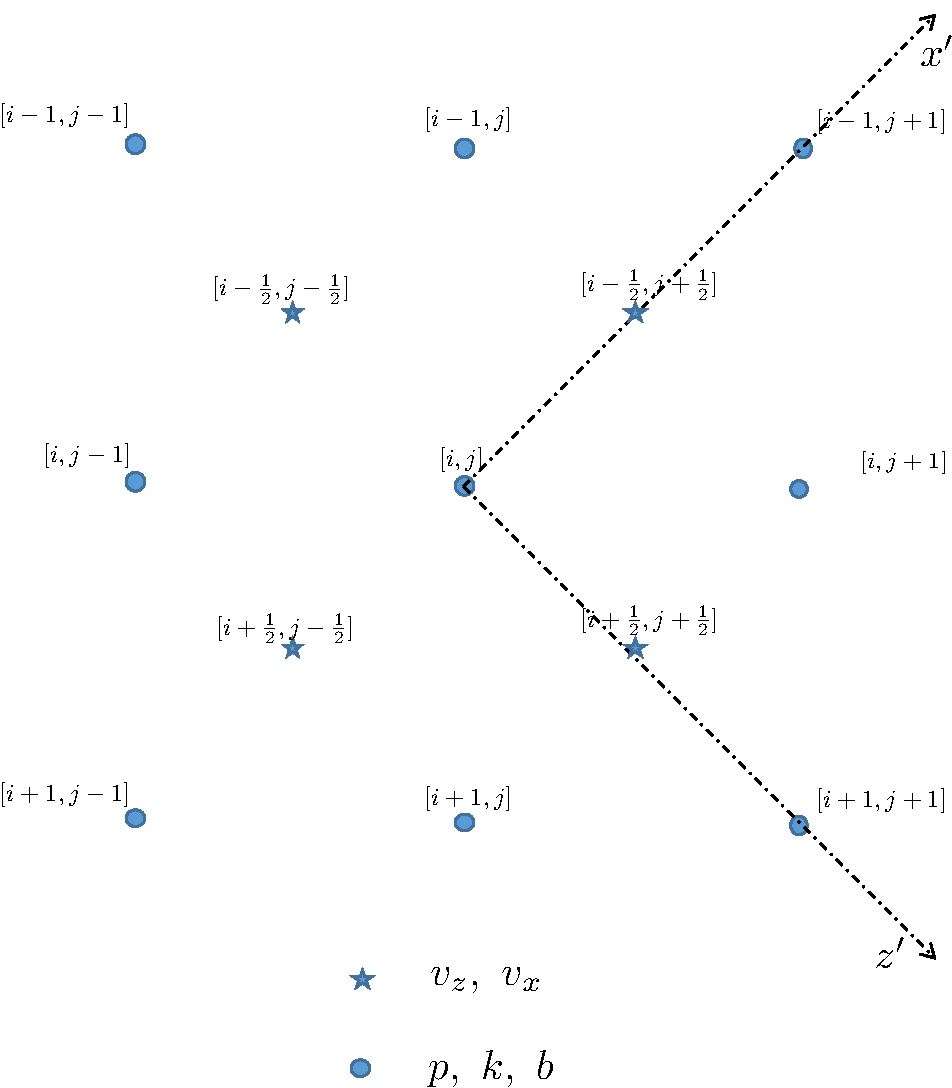
\includegraphics[width=0.6\columnwidth]{Fig/f2.pdf} 
   \caption{Rotated stagger grid}
   \label{f2}
\end{figure}

We first approximate the spatial partial derivative of partical velocity by finite difference, so we have
\begin{equation}
\begin{split}
\frac{\partial v_z}{\partial z^{\prime}}[i,j] &= \frac{v_z[i+\frac{1}{2},j+\frac{1}{2}] - v_z[i-\frac{1}{2},j-\frac{1}{2}] }{\sqrt{2}h} \\
\frac{\partial v_z}{\partial x^{\prime}}[i,j] &= \frac{v_z[i-\frac{1}{2},j+\frac{1}{2}] - v_z[i+\frac{1}{2},j-\frac{1}{2}] }{\sqrt{2}h} \\
\frac{\partial v_x}{\partial z^{\prime}}[i,j] &= \frac{v_x[i+\frac{1}{2},j+\frac{1}{2}] - v_x[i-\frac{1}{2},j-\frac{1}{2}] }{\sqrt{2}h} \\
\frac{\partial v_x}{\partial x^{\prime}}[i,j] &= \frac{v_x[i-\frac{1}{2},j+\frac{1}{2}] - v_x[i+\frac{1}{2},j-\frac{1}{2}] }{\sqrt{2}h} \\
\end{split} 
\label{eq103}
\end{equation}
From the first equation of the system \ref{eq88}:
\begin{equation}
iw v_z = \frac{\sqrt{2}}{2} \frac{b}{\epsilon_z} \left(\frac{\partial p}{\partial z^{\prime}} -\frac{\partial p}{\partial x^{\prime}} \right)
\label{eq104}
\end{equation}
we represent particle velocity component $v_z$ by pressure component $p$ as
\begin{equation}
\begin{split}
v_z[i-\frac{1}{2}, j-\frac{1}{2}] &= \frac{b[i-\frac{1}{2}, j-\frac{1}{2}]}{2h\, iw \epsilon_z[i-\frac{1}{2}]} \left(p[i,j] - p[i-1,j-1] + p[i,j-1] - p[i-1,j] \right) \\
v_z[i+\frac{1}{2}, j-\frac{1}{2}] &= \frac{b[i+\frac{1}{2}, j-\frac{1}{2}]}{2h\, iw \epsilon_z[i+\frac{1}{2}]} \left(p[i+1,j] - p[i,j-1] + p[i+1,j-1] - p[i,j] \right) \\
v_z[i-\frac{1}{2}, j+\frac{1}{2}] &= \frac{b[i-\frac{1}{2}, j+\frac{1}{2}]}{2h\, iw \epsilon_z[i-\frac{1}{2}]} \left(p[i,j+1] - p[i-1,j] + p[i,j] - p[i-1,j+1] \right) \\
v_z[i+\frac{1}{2}, j+\frac{1}{2}] &= \frac{b[i+\frac{1}{2}, j+\frac{1}{2}]}{2h\, iw \epsilon_z[i+\frac{1}{2}]} \left(p[i+1,j+1] - p[i,j] + p[i+1,j] - p[i,j+1] \right) \\
\end{split} 
\label{eq105}
\end{equation}
From the second equation of system \ref{eq88}:
\begin{equation}
iw v_x = \frac{\sqrt{2}}{2} \frac{b}{\epsilon_x} \left( \frac{\partial p}{\partial z^{\prime}} + \frac{\partial p}{\partial x^{\prime}}  \right)   
\label{eq106}
\end{equation}
By taking advantage of this equation, we can also represent $v_x$ via pressure component $p$ as:
\begin{equation}
\begin{split}
v_x[i-\frac{1}{2}, j-\frac{1}{2}] &= \frac{b[i-\frac{1}{2}, j-\frac{1}{2}]}{2h\, iw \epsilon_x[j-\frac{1}{2}]} \left(p[i,j] - p[i-1,j-1] + p[i-1,j] - p[i,j-1] \right) \\
v_x[i+\frac{1}{2}, j-\frac{1}{2}] &= \frac{b[i+\frac{1}{2}, j-\frac{1}{2}]}{2h\, iw \epsilon_x[j-\frac{1}{2}]} \left(p[i+1,j] - p[i,j-1] + p[i,j] - p[i+1,j-1] \right) \\
v_x[i-\frac{1}{2}, j+\frac{1}{2}] &= \frac{b[i-\frac{1}{2}, j+\frac{1}{2}]}{2h\, iw \epsilon_x[j+\frac{1}{2}]} \left(p[i,j+1] - p[i-1,j] + p[i-1,j+1] - p[i,j] \right) \\
v_x[i+\frac{1}{2}, j+\frac{1}{2}] &= \frac{b[i+\frac{1}{2}, j+\frac{1}{2}]}{2h\, iw \epsilon_x[j+\frac{1}{2}]} \left(p[i+1,j+1] - p[i,j] + p[i,j+1] - p[i+1,j] \right) \\
\end{split} 
\label{eq107}
\end{equation}
Summing the last two equations of the equation \ref{eq102}, we can get
\begin{equation}
\frac{iw}{k} p = \frac{\sqrt{2}}{2\epsilon_z} \left( \frac{\partial v_z}{\partial z^{\prime}} - \frac{\partial v_z}{\partial x^{\prime}} \right) + \frac{\sqrt{2}}{2\epsilon_x} \left( \frac{\partial v_x}{\partial z^{\prime}} + \frac{\partial v_x}{\partial x^{\prime}} \right) + \frac{f(w)}{k} 
\label{e108}
\end{equation}

Using the expressions in equation \ref{eq103}  to replace the terms in equation \ref{eq108}, we can get
\begin{equation}
\begin{split}
\frac{iw}{k[i,j]}p[i,j] & = \frac{1}{2h \epsilon_z[i]} \left( v_z[i+\frac{1}{2}, j+\frac{1}{2}] - v_z[i-\frac{1}{2},j-\frac{1}{2}] + v_z[i+\frac{1}{2}, j-\frac{1}{2}] - v_z[i-\frac{1}{2}, j+\frac{1}{2}] \right) \\
&+ \frac{1}{2h \epsilon_x[j]} \left(v_x[i+\frac{1}{2},j+\frac{1}{2}]- v_x[i-\frac{1}{2},j-\frac{1}{2}] + v_x[i-\frac{1}{2},j+\frac{1}{2}] - v_x[i+\frac{1}{2},j-\frac{1}{2}]\right) + \frac{f(w)}{k[i,j]} 
\end{split}
\label{eq109}
\end{equation}

The next step is to use the expression in equations (\ref{eq106}, \ref{eq107}) to replace the particle velocity terms in the equation \ref{eq109}. We also take out the terms $2h$ and $iw$,  then we can get a equation only with pressure component.
\begin{equation}
\begin{split}
\frac{-w^2}{k[i,j]}p[i,j] &= \frac{b[i+\frac{1}{2}, j+\frac{1}{2}]}{4h^2 \epsilon_z[i] \epsilon_z[i+\frac{1}{2}]} \left(p[i+1,j+1] - p[i,j] + p[i+1,j] - p[i,j+1] \right) \\
 &- \frac{b[i-\frac{1}{2}, j-\frac{1}{2}]}{4h^2 \epsilon_z[i] \epsilon_z[i-\frac{1}{2}]} \left(p[i,j] - p[i-1,j-1] + p[i,j-1] - p[i-1,j] \right) \\
 &+ \frac{b[i+\frac{1}{2}, j-\frac{1}{2}]}{4h^2 \epsilon_z[i] \epsilon_z[i+\frac{1}{2}]} \left(p[i+1,j] - p[i,j-1] + p[i+1,j-1] - p[i,j] \right) \\
 &- \frac{b[i-\frac{1}{2}, j+\frac{1}{2}]}{4h^2 \epsilon_z[i] \epsilon_z[i-\frac{1}{2}]} \left(p[i,j+1] - p[i-1,j] + p[i,j] - p[i-1,j+1] \right) \\
 &+ \frac{b[i+\frac{1}{2}, j+\frac{1}{2}]}{4h^2 \epsilon_x[j] \epsilon_x[j+\frac{1}{2}]} \left(p[i+1,j+1] - p[i,j] + p[i,j+1] - p[i+1,j] \right) \\
 &- \frac{b[i-\frac{1}{2}, j-\frac{1}{2}]}{4h^2 \epsilon_x[j] \epsilon_x[j-\frac{1}{2}]} \left(p[i,j] - p[i-1,j-1] + p[i-1,j] - p[i,j-1] \right) \\
 &+ \frac{b[i-\frac{1}{2}, j+\frac{1}{2}]}{4h^2 \epsilon_x[j] \epsilon_x[j+\frac{1}{2}]} \left(p[i,j+1] - p[i-1,j] + p[i-1,j+1] - p[i,j] \right) \\
 &- \frac{b[i+\frac{1}{2}, j-\frac{1}{2}]}{4h^2 \epsilon_x[j] \epsilon_x[j-\frac{1}{2}]} \left(p[i+1,j] - p[i,j-1] + p[i,j] - p[i+1,j-1] \right) \\
 &+ \frac{iw \,f(w)}{k[i,j]}
\end{split}
\label{eq110}
\end{equation}

To facilitate coding, we group the common terms in equation \ref{eq110} together, we get a new equations shown as bellow
\begin{equation}
\begin{split}
(\frac{-w^2}{k[i,j]} &+ \frac{b[i+\frac{1}{2}, j+\frac{1}{2}]}{4h^2 \epsilon_z[i] \epsilon_z[i+\frac{1}{2}]} + \frac{b[i-\frac{1}{2}, j-\frac{1}{2}]}{4h^2 \epsilon_z[i] \epsilon_z[i-\frac{1}{2}]} + \frac{b[i+\frac{1}{2}, j-\frac{1}{2}]}{4h^2 \epsilon_z[i] \epsilon_z[i+\frac{1}{2}]} + \frac{b[i-\frac{1}{2}, j+\frac{1}{2}]}{4h^2 \epsilon_z[i] \epsilon_z[i-\frac{1}{2}]} \\
                          &+ \frac{b[i+\frac{1}{2}, j+\frac{1}{2}]}{4h^2 \epsilon_x[j] \epsilon_x[j+\frac{1}{2}]} + \frac{b[i-\frac{1}{2}, j-\frac{1}{2}]}{4h^2 \epsilon_x[j] \epsilon_x[j-\frac{1}{2}]} + \frac{b[i-\frac{1}{2}, j+\frac{1}{2}]}{4h^2 \epsilon_x[j] \epsilon_x[j+\frac{1}{2}]} + \frac{b[i+\frac{1}{2}, j-\frac{1}{2}]}{4h^2 \epsilon_x[j] \epsilon_x[j-\frac{1}{2}]} ) p[i,j] \\
                          &- (\frac{b[i+\frac{1}{2}, j+\frac{1}{2}]}{4h^2 \epsilon_z[i] \epsilon_z[i+\frac{1}{2}]} + \frac{b[i+\frac{1}{2}, j+\frac{1}{2}]}{4h^2 \epsilon_x[j] \epsilon_x[j+\frac{1}{2}]}) p[i+1,j+1] \\
                          &- (\frac{b[i-\frac{1}{2}, j-\frac{1}{2}]}{4h^2 \epsilon_z[i] \epsilon_z[i-\frac{1}{2}]} + \frac{b[i-\frac{1}{2}, j-\frac{1}{2}]}{4h^2 \epsilon_x[j] \epsilon_x[j-\frac{1}{2}]})p[i-1,j-1]  \\
                          &- (\frac{b[i+\frac{1}{2}, j-\frac{1}{2}]}{4h^2 \epsilon_z[i] \epsilon_z[i+\frac{1}{2}]} + \frac{b[i+\frac{1}{2}, j-\frac{1}{2}]}{4h^2 \epsilon_x[j] \epsilon_x[j-\frac{1}{2}]})p[i+1,j-1] \\
                          &- (\frac{b[i-\frac{1}{2}, j+\frac{1}{2}]}{4h^2 \epsilon_z[i] \epsilon_z[i-\frac{1}{2}]} + \frac{b[i-\frac{1}{2}, j+\frac{1}{2}]}{4h^2 \epsilon_x[j] \epsilon_x[j+\frac{1}{2}]})p[i-1,j+1] \\
                          &-(\frac{b[i+\frac{1}{2}, j+\frac{1}{2}]}{4h^2 \epsilon_z[i] \epsilon_z[i+\frac{1}{2}]} +\frac{b[i+\frac{1}{2}, j-\frac{1}{2}]}{4h^2 \epsilon_z[i] \epsilon_z[i+\frac{1}{2}]} -\frac{b[i+\frac{1}{2}, j+\frac{1}{2}]}{4h^2 \epsilon_x[j] \epsilon_x[j+\frac{1}{2}]} -\frac{b[i+\frac{1}{2}, j-\frac{1}{2}]}{4h^2 \epsilon_x[j] \epsilon_x[j-\frac{1}{2}]} )p[i+1,j]  \\
                          &-(\frac{b[i-\frac{1}{2}, j+\frac{1}{2}]}{4h^2 \epsilon_x[j] \epsilon_x[j+\frac{1}{2}]} + \frac{b[i+\frac{1}{2}, j+\frac{1}{2}]}{4h^2 \epsilon_x[j] \epsilon_x[j+\frac{1}{2}]} - \frac{b[i+\frac{1}{2}, j+\frac{1}{2}]}{4h^2 \epsilon_z[i] \epsilon_z[i+\frac{1}{2}]} - \frac{b[i-\frac{1}{2}, j+\frac{1}{2}]}{4h^2 \epsilon_z[i] \epsilon_z[i-\frac{1}{2}]} )p[i,j+1] \\
                          &-(\frac{b[i-\frac{1}{2}, j-\frac{1}{2}]}{4h^2 \epsilon_x[j] \epsilon_x[j-\frac{1}{2}]} + \frac{b[i+\frac{1}{2}, j-\frac{1}{2}]}{4h^2 \epsilon_x[j] \epsilon_x[j-\frac{1}{2}]} - \frac{b[i-\frac{1}{2}, j-\frac{1}{2}]}{4h^2 \epsilon_z[i] \epsilon_z[i-\frac{1}{2}]} - \frac{b[i+\frac{1}{2}, j-\frac{1}{2}]}{4h^2 \epsilon_z[i] \epsilon_z[i+\frac{1}{2}]} )p[i,j-1] \\
                          &-(\frac{b[i-\frac{1}{2}, j-\frac{1}{2}]}{4h^2 \epsilon_z[i] \epsilon_z[i-\frac{1}{2}]} + \frac{b[i-\frac{1}{2}, j+\frac{1}{2}]}{4h^2 \epsilon_z[i] \epsilon_z[i-\frac{1}{2}]} - \frac{b[i-\frac{1}{2}, j-\frac{1}{2}]}{4h^2 \epsilon_x[j] \epsilon_x[j-\frac{1}{2}]} - \frac{b[i-\frac{1}{2}, j+\frac{1}{2}]}{4h^2 \epsilon_x[j] \epsilon_x[j+\frac{1}{2}]} )p[i-1,j] \\
                          &= \frac{iw\,f(w)}{k[i,j]}
\end{split} 
\label{eq111}
\end{equation}

\subsection{Mixed grid}
By combining the finte-difference grid based on Cartesian and the rotated coordinate system, we can get the mixed-grid finite-difference stencil. This process includes two steps:

\subsubsection{Connection between first order and second order Acoustic wave equation}
The first order acoustic wave equation is expressed  as
\begin{equation}
\begin{split}
 \frac{\partial v_z}{\partial t} &=  b \frac{\partial p}{\partial z}  \\
 \frac{\partial v_x}{\partial t} &=  b \frac{\partial p}{\partial x}  \\
\frac{\partial p}{\partial t} &= k \left(\frac{\partial v_z}{\partial z} + \frac{\partial v_x}{\partial x} \right) + f(t)
\end{split}
\label{in1}
\end{equation}
To derive the second order expression, we need to apply the time derivative to both side of the third equation expressed in equation \ref{in1}, we can get
\begin{equation}
\begin{split}
\frac{\partial^2 p}{\partial t^2} &= \frac{\partial}{\partial t}\left( k \left(\frac{\partial v_z}{\partial z} + \frac{\partial v_x}{\partial x} \right) \right) + \frac{\partial f(t)}{\partial t} \\
&=  k \left(\frac{\partial}{\partial z}\frac{\partial v_z}{\partial t} + \frac{\partial}{\partial x}\frac{\partial v_x}{\partial t} \right)  + \frac{\partial f(t)}{\partial t} 
\end{split}
\label{in2}
\end{equation}
As the model parameter $k$ is independent of time variable $t$ and exchange the order of 
partial derivative along time and spatial direction, next we are going to the expression in the first two equations of equation \ref{in1} to change the variable $\frac{\partial v_z}{\partial t}$ and  $\frac{\partial v_x}{\partial t}$, we can get
\begin{equation}
\frac{\partial^2 p}{\partial t^2} = k \left(  \frac{\partial}{\partial z} (b \frac{\partial p}{\partial z}) + \frac{\partial}{\partial x} (b \frac{\partial p}{\partial x})  \right) + \frac{\partial f(t)}{\partial t}
\label{in3}
\end{equation}
we can move the first term in the right hand side of equation \ref{in3} to the left hand side, dived by $k$, we get
\begin{equation}
\frac{1}{k}\frac{\partial^2 p}{\partial t^2} -  \left(  \frac{\partial}{\partial z} (b \frac{\partial p}{\partial z}) + \frac{\partial}{\partial x} (b \frac{\partial p}{\partial x})  \right) = \frac{1}{k}\frac{\partial f(t)}{\partial t}
\label{in4}
\end{equation}
The next step is to perform Fourier transform to frequency domain, we can get
\begin{equation}
\frac{-w^2}{k} p -  \left(  \frac{\partial}{\partial z} (b \frac{\partial p}{\partial z}) + \frac{\partial}{\partial x} (b \frac{\partial p}{\partial x})  \right) = \frac{iw f(w)}{k}
\label{in5}
\end{equation}

\subsubsection{Mass averaging}
\begin{equation}
\begin{split}
\frac{w^2}{k[i,j]}p[i,j] = w^2( &c \cdot \frac{p[i,j]}{k[i,j]} \\ 
+ &d (\frac{p[i+1,j]}{k[i+1,j]}+\frac{p[i-1,j]}{k[i-1,j]}+\frac{p[i,j+1]}{k[i,j+1]}+\frac{p[i,j-1]}{k[i,j-1]}) \\
+ & \frac{1-c-4d}{4} (\frac{p[i+1,j+1]}{k[i+1,j+1]}+\frac{p[i-1,j+1]}{k[i-1,j+1]}+\frac{p[i+1,j-1]}{k[i+1,j-1]}+ \frac{p[i-1,j-1]}{k[i-1,j-1]}) ) \\ 
\end{split}
\label{eq112}
\end{equation}

\subsubsection{Weighted averaging of the two stencil}
The weighting between the two grid is determined by parameter $\alpha$
\begin{equation}
-\frac{w^2}{k}p - a \cdot \left( \frac{\partial}{\partial z}(b \frac{\partial }{\partial z}) + \frac{\partial}{\partial x}(b \frac{\partial }{\partial x}) \right)p - (1-a) \cdot \left( \frac{\partial}{\partial z^{\prime}}(b\frac{\partial }{\partial z^{\prime}}) + \frac{\partial}{\partial x^{\prime}}(b \frac{\partial }{\partial x^{\prime}}) \right)p  = \frac{iw\, f(w)}{k}
\label{eq113}
\end{equation}
where $c=0.6287326$, $d=0.092816675$, $\alpha=0.5617365$. so the coefficient $\frac{1-c-4d}{4} = 1.75e-7$.
After some simple re-organzation of the terms, we give the coefficients for the 9 grid points
\begin{equation}
\begin{split}
p[i,j] \rightarrow -c \frac{w^2}{k[i,j]}+\alpha &\left\{  \frac{1}{\epsilon_z[i] h^2}\left(\frac{b[i+\frac{1}{2},j]}{\epsilon_z[i+\frac{1}{2}]} +  \frac{b[i-\frac{1}{2},j]}{\epsilon_z[i-\frac{1}{2}]} \right) + \frac{1}{\epsilon_x[j] h^2} \left( \frac{b[i,j+\frac{1}{2}]}{\epsilon_x[j+\frac{1}{2}]} + \frac{b[i,j-\frac{1}{2}]}{\epsilon_x[j-\frac{1}{2}]}\right) \right\} \\
 + (1-\alpha) &  \left\{    \frac{b[i+\frac{1}{2}, j+\frac{1}{2}]}{4h^2 \epsilon_z[i] \epsilon_z[i+\frac{1}{2}]}     +    \frac{b[i-\frac{1}{2}, j-\frac{1}{2}]}{4h^2 \epsilon_z[i] \epsilon_z[i-\frac{1}{2}]}      +       \frac{b[i+\frac{1}{2}, j-\frac{1}{2}]}{4h^2 \epsilon_z[i] \epsilon_z[i+\frac{1}{2}]}        + \frac{b[i-\frac{1}{2}, j+\frac{1}{2}]}{4h^2 \epsilon_z[i] \epsilon_z[i-\frac{1}{2}]}   \right\} \\
  + (1-\alpha) &  \left\{   \frac{b[i+\frac{1}{2}, j+\frac{1}{2}]}{4h^2 \epsilon_x[j] \epsilon_x[j+\frac{1}{2}]}     +    \frac{b[i-\frac{1}{2}, j-\frac{1}{2}]}{4h^2 \epsilon_x[j] \epsilon_x[j-\frac{1}{2}]}      +       \frac{b[i-\frac{1}{2}, j+\frac{1}{2}]}{4h^2 \epsilon_x[j] \epsilon_x[j+\frac{1}{2}]}    + \frac{b[i+\frac{1}{2}, j-\frac{1}{2}]}{4h^2 \epsilon_x[j] \epsilon_x[j-\frac{1}{2}]}      \right\}
\end{split}
\label{eq114}
\end{equation}

\begin{equation}
p[i-1,j-1] \rightarrow -\frac{1-c-4d}{4} \frac{w^2}{k[i-1,j-1]} - (1-\alpha) \left\{ \frac{b[i-\frac{1}{2}, j-\frac{1}{2}]}{4h^2 \epsilon_z[i] \epsilon_z[i-\frac{1}{2}]} + \frac{b[i-\frac{1}{2}, j-\frac{1}{2}]}{4h^2 \epsilon_x[j] \epsilon_x[j-\frac{1}{2}]}  \right\} \\
\label{eq115}
\end{equation}

\begin{equation}
\begin{split}
p[i,j-1] \rightarrow -d \frac{w^2}{k[i,j-1]} - \alpha &\frac{1}{\epsilon_x[j] h^2} \frac{b[i,j-\frac{1}{2}]}{\epsilon_x[j-\frac{1}{2}]}  \\
- (1-\alpha) &\left\{ \frac{b[i-\frac{1}{2}, j-\frac{1}{2}]}{4h^2 \epsilon_x[j] \epsilon_x[j-\frac{1}{2}]} + \frac{b[i+\frac{1}{2}, j-\frac{1}{2}]}{4h^2 \epsilon_x[j] \epsilon_x[j-\frac{1}{2}]} - \frac{b[i-\frac{1}{2}, j-\frac{1}{2}]}{4h^2 \epsilon_z[i] \epsilon_z[i-\frac{1}{2}]} - \frac{b[i+\frac{1}{2}, j-\frac{1}{2}]}{4h^2 \epsilon_z[i] \epsilon_z[i+\frac{1}{2}]} \right\} 
\end{split}
\label{eq116}
\end{equation}

\begin{equation}
p[i+1,j-1] \rightarrow -\frac{1-c-4d}{4} \frac{w^2}{k[i+1,j-1]} - (1-\alpha)\left\{\frac{b[i+\frac{1}{2}, j-\frac{1}{2}]}{4h^2 \epsilon_z[i] \epsilon_z[i+\frac{1}{2}]} + \frac{b[i+\frac{1}{2}, j-\frac{1}{2}]}{4h^2 \epsilon_x[j] \epsilon_x[j-\frac{1}{2}]} \right\} 
\label{eq117}
\end{equation}

\begin{equation}
\begin{split}
p[i-1,j] \rightarrow -d \frac{w^2}{k[i-1,j]} - \alpha &\left\{   \frac{1}{\epsilon_z[i] h^2} \frac{b[i-\frac{1}{2},j]}{\epsilon_z[i-\frac{1}{2}]}\right\} \\
- (1-\alpha) &\left\{   \frac{b[i-\frac{1}{2}, j-\frac{1}{2}]}{4h^2 \epsilon_z[i] \epsilon_z[i-\frac{1}{2}]} + \frac{b[i-\frac{1}{2}, j+\frac{1}{2}]}{4h^2 \epsilon_z[i] \epsilon_z[i-\frac{1}{2}]} - \frac{b[i-\frac{1}{2}, j-\frac{1}{2}]}{4h^2 \epsilon_x[j] \epsilon_x[j-\frac{1}{2}]} - \frac{b[i-\frac{1}{2}, j+\frac{1}{2}]}{4h^2 \epsilon_x[j] \epsilon_x[j+\frac{1}{2}]} \right\}
\end{split}
\label{eq118}
\end{equation}

\begin{equation}
\begin{split}
p[i+1,j] \rightarrow -d\frac{w^2}{k[i+1,j]} - \alpha &\left\{\frac{1}{\epsilon_z[i] h^2} \frac{b[i+\frac{1}{2},j]}{\epsilon_z[i+\frac{1}{2}]}\right\} \\
- (1-\alpha) &\left\{ \frac{b[i+\frac{1}{2}, j+\frac{1}{2}]}{4h^2 \epsilon_z[i] \epsilon_z[i+\frac{1}{2}]} +\frac{b[i+\frac{1}{2}, j-\frac{1}{2}]}{4h^2 \epsilon_z[i] \epsilon_z[i+\frac{1}{2}]} -\frac{b[i+\frac{1}{2}, j+\frac{1}{2}]}{4h^2 \epsilon_x[j] \epsilon_x[j+\frac{1}{2}]} -\frac{b[i+\frac{1}{2}, j-\frac{1}{2}]}{4h^2 \epsilon_x[j] \epsilon_x[j-\frac{1}{2}]} \right\}
\end{split} 
\label{eq119}
\end{equation}

\begin{equation}
p[i-1,j+1] \rightarrow -\frac{1-c-4d}{4} \frac{w^2}{k[i-1,j+1]} - (1-\alpha)\left\{\frac{b[i-\frac{1}{2}, j+\frac{1}{2}]}{4h^2 \epsilon_z[i] \epsilon_z[i-\frac{1}{2}]} + \frac{b[i-\frac{1}{2}, j+\frac{1}{2}]}{4h^2 \epsilon_x[j] \epsilon_x[j+\frac{1}{2}]}  \right\} 
\label{eq120}
\end{equation}

\begin{equation}
\begin{split}
p[i,j+1] \rightarrow -d\frac{w^2}{k[i,j+1]} - \alpha &\left\{  \frac{1}{\epsilon_x[j] h^2} \frac{b[i,j+\frac{1}{2}]}{\epsilon_x[j+\frac{1}{2}]}\right\} \\
- (1-\alpha) & \left\{  \frac{b[i-\frac{1}{2}, j+\frac{1}{2}]}{4h^2 \epsilon_x[j] \epsilon_x[j+\frac{1}{2}]} + \frac{b[i+\frac{1}{2}, j+\frac{1}{2}]}{4h^2 \epsilon_x[j] \epsilon_x[j+\frac{1}{2}]} - \frac{b[i+\frac{1}{2}, j+\frac{1}{2}]}{4h^2 \epsilon_z[i] \epsilon_z[i+\frac{1}{2}]} - \frac{b[i-\frac{1}{2}, j+\frac{1}{2}]}{4h^2 \epsilon_z[i] \epsilon_z[i-\frac{1}{2}]}  \right\}
\end{split}
\label{eq121}
\end{equation}

\begin{equation}
p[i+1,j+1] \rightarrow -\frac{1-c-4d}{4} \frac{w^2}{k[i+1,j+1]} - (1-\alpha)\left\{\frac{b[i+\frac{1}{2}, j+\frac{1}{2}]}{4h^2 \epsilon_z[i] \epsilon_z[i+\frac{1}{2}]} + \frac{b[i+\frac{1}{2}, j+\frac{1}{2}]}{4h^2 \epsilon_x[j] \epsilon_x[j+\frac{1}{2}]}  \right\}
\label{eq122}
\end{equation}

Outside of PML area, $\epsilon_z=\epsilon_x=1$, the above coefficients can be simplified as 
\begin{equation}
\begin{split}
p[i,j] \rightarrow & -c\frac{w^2}{k[i,j]} + \frac{a}{h^2}( b[i+\frac{1}{2},j]+ b[i-\frac{1}{2},j]+b[i,j+\frac{1}{2}]+b[i,j-\frac{1}{2}]) \\
  & + \frac{1-a}{2h^2}(b[i+\frac{1}{2},j+\frac{1}{2}]+b[i-\frac{1}{2},j-\frac{1}{2}]+b[i-\frac{1}{2},j+\frac{1}{2}]+b[i+\frac{1}{2},j-\frac{1}{2}]) \\
 p[i-1,j-1] \rightarrow & -\frac{1-c-4d}{4} \frac{w^2}{k[i-1,j-1]} -  \frac{1-a}{2h^2}b[i-\frac{1}{2},j-\frac{1}{2}] \\
 p[i,j-1]   \rightarrow & -d \frac{w^2}{k[i,j-1]} - \frac{\alpha}{h^2} b[i,j-\frac{1}{2}] \\
 p[i+1,j-1] \rightarrow & -\frac{1-c-4d}{4} \frac{w^2}{k[i+1,j-1]} - \frac{1-a}{2h^2}b[i+\frac{1}{2},j-\frac{1}{2}] \\
 p[i-1,j]   \rightarrow & -d\frac{w^2}{k[i-1,j]} - \frac{\alpha}{h^2} b[i-\frac{1}{2},j] \\
 p[i+1,j]   \rightarrow & -d\frac{w^2}{k[i+1,j]}  - \frac{\alpha}{h^2} b[i+\frac{1}{2},j] \\
 p[i-1,j+1] \rightarrow & -\frac{1-c-4d}{4} \frac{w^2}{k[i-1,j+1]} -\frac{1-a}{2h^2}b[i-\frac{1}{2},j+\frac{1}{2}] \\
 p[i,j+1]   \rightarrow & -d\frac{w^2}{k[i,j+1]} - \frac{\alpha}{h^2} b[i,j+\frac{1}{2}] \\
 p[i+1,j+1] \rightarrow & -\frac{1-c-4d}{4} \frac{w^2}{k[i+1,j+1]} - \frac{1-a}{2h^2}b[i+\frac{1}{2},j+\frac{1}{2}] \\
\end{split}
\label{eq123}
\end{equation}
The expression in equation \ref{eq123} can be used to derive the gradient of FWI for model parameters. The source wavelet is add as 
\begin{equation}
\frac{iw f(w)}{k[i,j]}\,,
\label{eq124}
\end{equation}
where $[i,j]$ indicate the location of source point.

\subsection{Gradient for FWI in frequency domain}
Based on above formulations, we can create the Helmholtz operator as an sparse matrix ${\bf H}$, so the forward modelling process can be expressed as
\begin{equation}
{{\bf H}({\bf m}) \, {\bf u}({\bf m}) = {\bf f}}
\label{eq125}
\end{equation}
where ${\bf H}$ is the Helmholtz operator and ${\bf m}$ is model parameter, ${\bf u}$ is the wave field at one frequency component and ${\bf f}$ is the source signature in the frequency domain. Follow the notations we used for time-domain finite difference method, the size of ${\bf H}$ is $N_z\cdot N_x \times N_z\cdot N_x$. The wave field at one frequency slice ${\bf u}$ is a vector length of $N_z \cdot N_x$, so as to the source signature ${\bf f}$.

To simplify the derivations of gradient, we temporarily just consider one frequency slice. The synthetic data is obtained by sampling the wave field at the receiver's location, the sampling operator is indicated by operator ${\bf S}$. So the synthetic data is represented as 
\begin{equation}
{\bf d = Su}
\label{eq126}
\end{equation}
In FWI, the model parameter is updated by minimizing the difference between the synthetic and observed data, here we just use the $l2$ norm as the metric to evaluate the difference, so the objective function is given as 
\begin{equation}
J = \frac{1}{2}||{\bf d} - {\bf d}_{obs}||_2^2 = \frac{1}{2}({\bf d} - {\bf d}_{obs})^T ({\bf d} - {\bf d}_{obs})^*
\label{eq127}
\end{equation}
Where ${\bf d}_{obs}$ is the observed data, the symbol $^T$ and $^*$ represent matrix transpose and complex conjugate. We assume the density is constant, so the model parameter is just the velocity model.

We derive the derivative of the cost with respect to one model parameter $m_l$, $l$ is the linear index of this model parameter. The derivative is given as 
\begin{equation}
\frac{\partial J}{\partial m_l} = \left( \frac{\partial {\bf u}}{\partial m_l} \right)^T \frac{\partial J}{\partial {\bf u}} + \left( \frac{\partial {\bf u^*}}{\partial m_l} \right)^T \frac{\partial J}{\partial {\bf u^*}}
\label{eq128}
\end{equation}
Base on the equation \ref{eq125}, \ref{eq126}, using the property of complex conjugate, we can get
\begin{equation}
\begin{split}
{\bf H}^*({\bf m}) \, {\bf u}^*({\bf m})& = {\bf f}^* \\
{\bf d}^* &= {\bf S}^*{\bf u}^*
\end{split}
\label{eq129}
\end{equation}
We take the derivative of equation \ref{eq125} and \ref{eq129} with respect to $m_l$, we get 
\begin{equation}
\begin{split}
\frac{\partial }{\partial m_l} \left({\bf Hu} \right) &= \frac{\partial {\bf f}}{\partial m_l} \\
\frac{\partial }{\partial m_l} \left({\bf H}^* {\bf u}^* \right) &= \frac{\partial {\bf f}^*}{\partial m_l} \\
\end{split}
\label{eq130}
\end{equation}
As the source signature is independent of model parameter ${\bf m}$, the expression shows in equation \ref{eq130} can be simplified as
\begin{equation}
\begin{split}
\frac{\partial {\bf H}}{\partial m_l} {\bf u} + {\bf H} \frac{\partial {\bf u}}{\partial m_l}&= {\bf 0}\\
\frac{\partial {\bf H}^*}{\partial m_l} {\bf u}^* + {\bf H}^* \frac{\partial {\bf u}^*}{\partial m_l}&= {\bf 0}\\
\end{split}
\label{eq131}
\end{equation}
So we can get the expression of $\frac{\partial {\bf u}}{\partial m_l}$ and $\frac{\partial {\bf u}^*}{\partial m_l}$, which are given as 
\begin{equation}
\begin{split}
\frac{\partial {\bf u}}{\partial m_l}&= - {\bf H}^{-1} \,\frac{\partial {\bf H}}{\partial m_l} {\bf u} \\
\frac{\partial {\bf u}^*}{\partial m_l}&=  -\left({\bf H}^*\right)^{-1}  \, \frac{\partial {\bf H}^*}{\partial m_l} {\bf u}^*\\
\end{split}
\label{eq132}
\end{equation}
The next step we need to figure out the expression of $\frac{\partial J}{\partial {\bf u}}$ and $\frac{\partial J}{\partial {\bf u}^*}$. As equation \ref{eq127} can be also written as
\begin{equation}
J = \frac{1}{2}({\bf S}{\bf u} - {\bf d}_{obs})^T ({\bf S}{\bf u}^* - {\bf d}_{obs}^*)
\label{eq133}
\end{equation}
It is easy to derive that
\begin{equation}
\begin{split}
\frac{\partial J}{\partial {\bf u}} & = \frac{1}{2} {\bf S}^T ({\bf d}^* - {\bf d}_{obs}^*) \\
\frac{\partial J}{\partial {\bf u}^*} & = \frac{1}{2} {\bf S}^T ({\bf d} - {\bf d}_{obs}) \\
\end{split}
\label{eq134}
\end{equation}
We combine the result of equation \ref{eq128}, \ref{eq132} and \ref{eq134}, we can get
\begin{equation}
\begin{split}
\frac{\partial J}{\partial m_l} &= -\frac{1}{2} \left(    \left({\bf H}^{-1} \,\frac{\partial {\bf H}}{\partial m_l} {\bf u}\right)^T {\bf S}^T ({\bf d}^* - {\bf d}_{obs}^*)  + \left( \left({\bf H}^*\right)^{-1}  \, \frac{\partial {\bf H}^*}{\partial m_l} {\bf u}^*\right)^T  {\bf S}^T ({\bf d} - {\bf d}_{obs})   \right) \\
 &= -\frac{1}{2} \left(    \left({\bf H}^{-1} \,\frac{\partial {\bf H}}{\partial m_l} {\bf u}\right)^T {\bf S}^T ({\bf d}^* - {\bf d}_{obs}^*)  + \left( \left({\bf H}^{-1}\right)^*  \, \frac{\partial {\bf H}^*}{\partial m_l} {\bf u}^*\right)^T  {\bf S}^T ({\bf d} - {\bf d}_{obs})   \right) \\
  &= -\frac{1}{2} \left(    \left({\bf H}^{-1} \,\frac{\partial {\bf H}}{\partial m_l} {\bf u}\right)^T {\bf S}^T ({\bf d}^* - {\bf d}_{obs}^*)  + \left( \left( {\bf H}^{-1}  \, \frac{\partial {\bf H}}{\partial m_l} {\bf u} \right)^T \right)^* {\bf S}^T ({\bf d} - {\bf d}_{obs})   \right)
\end{split}
\label{eq135}
\end{equation}
It is not easily to find that the second term is the complex conjugate of the first term in the above equation. So the final form of the gradient can be simplified as
\begin{equation}
\begin{split}
\frac{\partial J}{\partial m_l} &= -{\mathcal R} \left\{    \left({\bf H}^{-1} \,\frac{\partial {\bf H}}{\partial m_l} {\bf u}\right)^T {\bf S}^T ({\bf d}^* - {\bf d}_{obs}^*)  \right\} \\
&= -{\mathcal R} \left\{  \left( \frac{\partial {\bf H}}{\partial m_l} {\bf u} \right)^T  ({\bf H}^T)^{-1} \,    {\bf S}^T ({\bf d}^* - {\bf d}_{obs}^*)  \right\} \\
\end{split}
\label{eq136}
\end{equation}
where ${\mathcal R}$ is the operator which take the real part of complex number. People usually call $\left( \frac{\partial {\bf H}}{\partial m_l} {\bf u} \right)$ as the source side wave field and $({\bf H}^T)^{-1} \,    {\bf S}^T ({\bf d}^* - {\bf d}_{obs}^*)$ as adjoint wave field, the gradient is obtained by the inner product between source-side wave field and adjoint wave field.

We considering the details of $\frac{\partial {\bf H}}{\partial m_l}$, we temporarily only consider the velocity as the model parameter and consider density as constant (not updated by inversion). To simplify the derivation, we assume the model size (include PML) is $3 \times 4$.
The mapping between sub-index and linear index are expressed as follow
\begin{equation}
\begin{pmatrix}
[1,1] \rightarrow 1 & [1,2] \rightarrow 4 & [1,3]\rightarrow 7 & [1,4]\rightarrow 10 \\
[2,1]\rightarrow 2 & [2,2]\rightarrow 5   & [2,3]\rightarrow 8 & [2,4]\rightarrow 11 \\
[3,1]\rightarrow 3 & [3,2] \rightarrow 6  & [3,3]\rightarrow 9 & [3,4]\rightarrow 12 \\
\end{pmatrix}
\end{equation}
We only consider the velocity part and define $c_1 = -c\, \omega^2$, $c_2 = - d\,\omega^2$, $c_3 = - \frac{1-c-4d}{4}\,\omega^2$
 So the part of the Hessian matrix only related to velocity model can be expressed as
\begin{equation}
\begin{pmatrix}
\frac{c_1}{k_1} & \frac{c_2}{k_2} & \quad & \frac{c_2}{k_4} & \frac{c_3}{k_5} & \quad & \quad & \quad & \quad & \quad & \quad & \quad \\

\frac{c_2}{k_1} & \frac{c_1}{k_2} & \frac{c_2}{k_3} & \frac{c_3}{k_4} & \frac{c_2}{k_5} & \frac{c_3}{k_6}  & \quad & \quad & \quad & \quad & \quad & \quad \\

\quad & \frac{c_2}{k_2} & \frac{c_1}{k_3} & \quad & \frac{c_3}{k_5} & \frac{c_2}{k_6}  & \quad & \quad & \quad & \quad & \quad & \quad \\\\

\frac{c_2}{k_1} & \frac{c_3}{k_2}  & \quad & \frac{c_1}{k_4}  & \frac{c_2}{k_5} & \quad   & \frac{c_2}{k_7} & \frac{c_3}{k_8} & \quad & \quad & \quad & \quad \\

\frac{c_3}{k_1} & \frac{c_2}{k_2} & \frac{c_3}{k_3} & \frac{c_2}{k_4} & \frac{c_1}{k_5} & \frac{c_2}{k_6} & \frac{c_3}{k_7} & \frac{c_2}{k_8} & \frac{c_3}{k_9} & \quad & \quad & \quad \\

\quad & \frac{c_3}{k_2} & \frac{c_2}{k_3} &  \quad & \frac{c_2}{k_5} & \frac{c_1}{k_6} &  \quad & \frac{c_3}{k_8} & \frac{c_2}{k_9} &  \quad &  \quad &  \quad \\\\

\quad & \quad &\quad & \frac{c_2}{k_4]} & \frac{c_3}{k_5} & \quad & \frac{c_1}{k_7} & \frac{c_2}{k_8} & \quad & \frac{c_2}{k_{10}} & \frac{c_3}{k_{11}} & \quad \\

\quad  & \quad  & \quad & \frac{c_3}{k_4} & \frac{c_2}{k_5} & \frac{c_3}{k_6} & \frac{c_2}{k_7}  & \frac{c_1}{k_8} & \frac{c_2}{k_9}  & \frac{c_3}{k_{10}} & \frac{c_2}{k_{11}} & \frac{c_3}{k_{12}} \\

\quad &  \quad &  \quad &  \quad & \frac{c_3}{k_5} & \frac{c_2}{k_6} &  \quad & \frac{c_2}{k_8} & \frac{c_1}{k_9} &  \quad & \frac{c_3}{k_{11}} & \frac{c_2}{k_{12}} \\\\

\quad &  \quad &  \quad & \quad & \quad & \quad & \frac{c_2}{k_7} & \frac{c_3}{k_8} & \quad & \frac{c_1}{k_{10}} & \frac{c_2}{k_{11}} & \quad \\
 
\quad &  \quad &  \quad & \quad & \quad & \quad & \frac{c_3}{k_7} & \frac{c_2}{k_8} & \frac{c3}{k_9} & \frac{c_2}{k_{10}} & \frac{c_1}{k_{11}} & \frac{c_2}{k_{12}} \\

\quad &  \quad &  \quad & \quad & \quad & \quad & \quad & \frac{c_3}{k[_8} & \frac{c_2}{k_9} & \quad & \frac{c_2}{k_{11}} & \frac{c_1}{k_{12}} 
\end{pmatrix}
\end{equation}
We know $k = \rho \times v^2$, so $\frac{\partial \frac{c_i}{k}}{\partial\, v} = -\frac{2\, c_i \rho v}{k^2} =  -\frac{2\, c_i}{\rho v^3}$
Suppose we want to compute $\frac{\partial {\bf H}}{\partial v_5}$ is given as
\begin{equation}
\begin{pmatrix}
0 & 0 & 0 & 0 & -\frac{2\, c_3}{\rho_5 v_5^3} & 0 & 0 & 0 & 0 & 0 & 0 & 0 \\
0 & 0 & 0 & 0 & -\frac{2\, c_2}{\rho_5 v_5^3} & 0 & 0 & 0 & 0 & 0 & 0 & 0 \\
0 & 0 & 0 & 0 & -\frac{2\, c_3}{\rho_5 v_5^3} & 0 & 0 & 0 & 0 & 0 & 0 & 0 \\
0 & 0 & 0 & 0 & -\frac{2\, c_2}{\rho_5 v_5^3} & 0 & 0 & 0 & 0 & 0 & 0 & 0 \\
0 & 0 & 0 & 0 & -\frac{2\, c_1}{\rho_5 v_5^3} & 0 & 0 & 0 & 0 & 0 & 0 & 0 \\
0 & 0 & 0 & 0 & -\frac{2\, c_2}{\rho_5 v_5^3} & 0 & 0 & 0 & 0 & 0 & 0 & 0 \\
0 & 0 & 0 & 0 & -\frac{2\, c_3}{\rho_5 v_5^3} & 0 & 0 & 0 & 0 & 0 & 0 & 0 \\
0 & 0 & 0 & 0 & -\frac{2\, c_2}{\rho_5 v_5^3} & 0 & 0 & 0 & 0 & 0 & 0 & 0 \\
0 & 0 & 0 & 0 & -\frac{2\, c_3}{\rho_5 v_5^3} & 0 & 0 & 0 & 0 & 0 & 0 & 0 \\
0 & 0 & 0 & 0 & 0 & 0 & 0 & 0 & 0 & 0 & 0 & 0 \\
0 & 0 & 0 & 0 & 0 & 0 & 0 & 0 & 0 & 0 & 0 & 0 \\
0 & 0 & 0 & 0 & 0 & 0 & 0 & 0 & 0 & 0 & 0 & 0 \\
\end{pmatrix}
\end{equation}
So the result of $\left( \frac{\partial {\bf H}}{\partial v_5} {\bf u} \right)$ is given as
\begin{equation}
\begin{pmatrix}
0 & 0 & 0 & 0 & -\frac{2\, c_3}{\rho_5 v_5^3} & 0 & 0 & 0 & 0 & 0 & 0 & 0 \\
0 & 0 & 0 & 0 & -\frac{2\, c_2}{\rho_5 v_5^3} & 0 & 0 & 0 & 0 & 0 & 0 & 0 \\
0 & 0 & 0 & 0 & -\frac{2\, c_3}{\rho_5 v_5^3} & 0 & 0 & 0 & 0 & 0 & 0 & 0 \\
0 & 0 & 0 & 0 & -\frac{2\, c_2}{\rho_5 v_5^3} & 0 & 0 & 0 & 0 & 0 & 0 & 0 \\
0 & 0 & 0 & 0 & -\frac{2\, c_1}{\rho_5 v_5^3} & 0 & 0 & 0 & 0 & 0 & 0 & 0 \\
0 & 0 & 0 & 0 & -\frac{2\, c_2}{\rho_5 v_5^3} & 0 & 0 & 0 & 0 & 0 & 0 & 0 \\
0 & 0 & 0 & 0 & -\frac{2\, c_3}{\rho_5 v_5^3} & 0 & 0 & 0 & 0 & 0 & 0 & 0 \\
0 & 0 & 0 & 0 & -\frac{2\, c_2}{\rho_5 v_5^3} & 0 & 0 & 0 & 0 & 0 & 0 & 0 \\
0 & 0 & 0 & 0 & -\frac{2\, c_3}{\rho_5 v_5^3} & 0 & 0 & 0 & 0 & 0 & 0 & 0 \\
0 & 0 & 0 & 0 & 0 & 0 & 0 & 0 & 0 & 0 & 0 & 0 \\
0 & 0 & 0 & 0 & 0 & 0 & 0 & 0 & 0 & 0 & 0 & 0 \\
0 & 0 & 0 & 0 & 0 & 0 & 0 & 0 & 0 & 0 & 0 & 0 \\
\end{pmatrix}
\begin{bmatrix}
u_1\\
u_2\\
u_3\\
u_4\\
u_5\\
u_6\\
u_7\\
u_8\\
u_9\\
u_{10}\\
u_{11}\\
u_{12}\\
\end{bmatrix}
=
\begin{bmatrix}
-\frac{2\, c_3\, u_5}{\rho_5 v_5^3} \\
-\frac{2\, c_2\, u_5}{\rho_5 v_5^3} \\
-\frac{2\, c_3\, u_5}{\rho_5 v_5^3} \\
-\frac{2\, c_2\, u_5}{\rho_5 v_5^3} \\
-\frac{2\, c_1\, u_5}{\rho_5 v_5^3} \\
-\frac{2\, c_2\, u_5}{\rho_5 v_5^3}  \\
-\frac{2\, c_3\, u_5}{\rho_5 v_5^3} \\
-\frac{2\, c_2\, u_5}{\rho_5 v_5^3}  \\
-\frac{2\, c_3\, u_5}{\rho_5 v_5^3} \\
0 \\
0 \\
0 \\
\end{bmatrix}
=
-\frac{2\, u_5}{\rho_5 \,v_5^3}
\begin{bmatrix}
c_3 \\
c_2 \\
c_3 \\
c_2 \\
c_1 \\
c_2 \\
c_3 \\
c_2 \\
c_3 \\
0 \\
0 \\
0 \\
\end{bmatrix}
\end{equation}
We also name the adjoint wave field is given as
\begin{equation}
{\bf u}_{adj} = ({\bf H}^T)^{-1} \,    {\bf S}^T ({\bf d}^* - {\bf d}_{obs}^*)
\end{equation}
The final formulation of the gradient of $v_5$ is given as
\begin{equation}
\begin{split}
g_5 &= \left( \frac{\partial {\bf H}}{\partial v_5} {\bf u} \right)^T \tilde{\bf u} \\
       &= -\frac{2\, u_5}{\rho_5 \,v_5^3} \begin{bmatrix}
       c_3 &
c_2 &
c_3 &
c_2 &
c_1 &
c_2 &
c_3 &
c_2 &
c_3 &
0 &
0 &
0 
\end{bmatrix}
\begin{bmatrix}
\tilde{u}_1 \\
\tilde{u}_2 \\
\tilde{u}_3 \\
\tilde{u}_4 \\
\tilde{u}_5 \\
\tilde{u}_6 \\
\tilde{u}_7 \\
\tilde{u}_8 \\
\tilde{u}_9 \\
0 \\
0 \\
0 \\
\end{bmatrix}
\end{split}
\end{equation}



%\bibliographystyle{seg}
%\bibliography{paper}

\end{document}

